% Chương 2: Cơ sở lý thuyết và tổng quan
\chapter{CƠ SỞ LÝ THUYẾT VÀ TỔNG QUAN}

Chương này xây dựng cơ sở lý thuyết cho kiến trúc được đề xuất ở Chương 3. Nội dung được tổ chức theo hướng đi từ bài toán tới công cụ, rồi từ công cụ tới giới hạn của chúng.

Bốn mục đầu xác lập nền. Mục 2.1 xác định những thuộc tính nào làm cho một văn bằng số trở nên đáng tin cậy. Mục 2.2 phân tích các mô hình quản lý định danh và lý do mô hình định danh tự chủ được lựa chọn. Mục 2.3 trình bày các khối kiến trúc kỹ thuật, và Mục 2.4 trình bày các nguyên thủy mật mã hiện thực hóa chúng.

Mục 2.5 làm rõ vai trò của blockchain, và làm rõ theo cả hai chiều: vai trò đó hẹp hơn thường được mô tả, và nó phải được biện minh thay vì mặc định. Vì vậy mục này có hai phần phản biện --- một phần đối chiếu với các phương án thay thế không dùng blockchain, và một phần xem xét ràng buộc từ quy định về bảo vệ dữ liệu cá nhân, vốn đặt câu hỏi nghiêm trọng với chính cách tiếp cận neo giá trị băm lên chuỗi công khai.

Mục 2.6 trình bày lăng kính phân tích của chương: phân tầng khái niệm niềm tin, qua đó định vị chính xác tầng nào mật mã học không thể giải quyết. Mục 2.7 khảo sát các hệ thống hiện có dưới lăng kính đó, bao gồm hai phân tích an toàn cho thấy khoảng trống về thẩm quyền đã thực sự bị khai thác trên các hệ thống đã triển khai. Mục 2.8 phân loại khoảng trống nghiên cứu thành sáu tầng và xác định tầng nào thuộc phạm vi can thiệp của khóa luận --- kể cả tầng mà khóa luận không xử lý được.

\section{Văn bằng số và các thuộc tính của sự tin cậy}

\subsection{Ba thế hệ biểu diễn văn bằng}

Việc phân biệt ba thế hệ biểu diễn văn bằng giúp xác định chính xác điều gì thay đổi và điều gì không thay đổi qua mỗi bước chuyển.

\textbf{Thế hệ thứ nhất là văn bằng vật lý.} Tính xác thực dựa trên các đặc trưng khó sao chép của vật thể: con dấu nổi, giấy có hoa văn bảo an, chữ ký tay, mực đặc biệt. Việc kiểm chứng dựa trên hai nguồn: quan sát trực tiếp các đặc trưng vật lý, và đối chiếu với sổ gốc do cơ sở cấp phát lưu giữ. Cả hai nguồn đều có hạn chế. Quan sát trực tiếp đòi hỏi chuyên môn mà bên xác minh thường không có, còn đối chiếu sổ gốc thì phụ thuộc hoàn toàn vào bên cấp phát.

\textbf{Thế hệ thứ hai là văn bằng số hóa.} Văn bằng được chuyển sang tệp PDF, ảnh quét, hoặc một bản ghi trong cơ sở dữ liệu trực tuyến. Khả năng lưu trữ và phân phối được cải thiện rõ rệt, nhưng cơ chế thiết lập niềm tin thì không. Một tệp PDF có thể bị chỉnh sửa, và một bản ghi trả về từ cổng tra cứu chỉ đáng tin trong chừng mực bên xác minh tin vào tổ chức vận hành cổng đó. Thế hệ này số hóa \emph{hình thức biểu diễn} của văn bằng mà không số hóa \emph{cơ chế xác thực} gắn liền với nó --- đó là lý do nó không giải quyết được ba hệ quả kiến trúc đã nêu tại Mục 1.1.3.

\textbf{Thế hệ thứ ba số hóa chính bằng chứng về tính xác thực.} Thông tin đủ để kiểm chứng được nhúng vào cấu trúc của văn bằng: một chữ ký số trên toàn bộ nội dung, một tham chiếu tới nơi tra được khóa công khai của bên ký, và một tham chiếu tới nơi tra được trạng thái hiệu lực. Bên xác minh thực hiện phép kiểm tra bằng toán học trên dữ liệu mình đang giữ, thay vì gửi câu hỏi đến bên cấp phát. Sự chuyển dịch ở đây là từ \emph{niềm tin vào trung gian} sang \emph{niềm tin vào bằng chứng}, và đó mới là thay đổi mang tính kiến trúc.

Cần nhấn mạnh rằng thế hệ thứ ba không loại bỏ vai trò của tổ chức. Nó chỉ thay đổi thời điểm và cách thức tổ chức tham gia: thay vì tham gia vào \emph{từng} lần xác minh, tổ chức tham gia \emph{một lần} vào thời điểm phát hành, và tham gia vào việc duy trì trạng thái. Chi phí của một lần xác minh vì thế không còn tỉ lệ với số lần xác minh.

\subsection{Ba thuộc tính của một văn bằng số đáng tin cậy}

Từ góc độ hệ thống, một văn bằng số chỉ có thể được coi là đáng tin cậy khi đồng thời bảo đảm ba thuộc tính độc lập nhau. Ba thuộc tính dưới đây được tổng hợp từ mô hình dữ liệu chứng thực của W3C \cite{W3C_VCDM2025} và từ các tài liệu nền về định danh tự chủ \cite{Preukschat2021, Sedlmeir2021}; cách phát biểu và việc nhấn mạnh tính độc lập giữa chúng là của nghiên cứu này, nhằm phục vụ phần phân tích ngay sau đó.

\begin{itemize}
    \item \textbf{Xác thực nguồn gốc.} Văn bằng chứng minh được nó do một thực thể xác định phát hành, và bên xác minh kiểm chứng được điều này mà không cần liên hệ với thực thể đó. Thuộc tính này được hiện thực hóa bằng chữ ký số cùng cơ chế công bố khóa công khai.
    \item \textbf{Toàn vẹn nội dung.} Dữ liệu không bị thay đổi sau thời điểm phát hành, và mọi chỉnh sửa --- kể cả thay đổi một ký tự --- đều bị phát hiện. Thuộc tính này được hiện thực hóa bằng hàm băm mật mã kết hợp với một cam kết đã công bố trước.
    \item \textbf{Trạng thái hiệu lực theo thời gian.} Văn bằng phản ánh được trạng thái của nó tại thời điểm xác minh, bao gồm các trường hợp bị thu hồi, tạm đình chỉ hoặc hết hạn.
\end{itemize}

Ba thuộc tính này không thay thế được nhau, và sự độc lập của chúng có hệ quả thiết kế trực tiếp. Chữ ký số bảo đảm thuộc tính thứ nhất và thứ hai \emph{tại thời điểm ký}, nhưng không nói gì về thuộc tính thứ ba: một văn bằng đã bị thu hồi vì gian lận vẫn mang chữ ký hoàn toàn hợp lệ về mặt toán học. Ngược lại, một hệ thống chỉ theo dõi trạng thái --- trả lời được {``}văn bằng này còn hiệu lực không{''} --- lại không phát hiện được trường hợp nội dung bị sửa sau khi cấp, bởi trạng thái của bản ghi vẫn là {``}đang hiệu lực{''}. Đây không phải lỗ hổng lý thuyết: Mục 3.6 và 4.7 cho thấy một quy trình xác minh thiếu bước đối chiếu nội dung với giá trị băm đã neo sẽ bỏ sót đúng loại tấn công này.

Thuộc tính thứ tư, không nằm trong danh sách trên nhưng quyết định giá trị thực tế của văn bằng, là \emph{thẩm quyền của bên phát hành}. Đây là thuộc tính thuộc tầng khác và sẽ được phân tích riêng tại Mục 2.6.

\section{Định danh số và các mô hình quản lý định danh}

\subsection{Phân biệt danh tính số và định danh số}

Hai khái niệm thường bị dùng lẫn nhưng có vai trò khác biệt trong kiến trúc.

Theo hướng dẫn của Viện Tiêu chuẩn và Công nghệ Quốc gia Hoa Kỳ, \textbf{danh tính số} (digital identity) là biểu diễn dưới dạng số của một tập hợp thuộc tính về một chủ thể, được sử dụng trong bối cảnh giao dịch điện tử \cite{NIST_SP800_63_3}. Windley bổ sung một quan sát quan trọng cho kiến trúc: danh tính không phải một thực thể cố định mà là tập hợp thuộc tính phù hợp với một ngữ cảnh cụ thể, nên cùng một người tồn tại dưới nhiều danh tính số khác nhau tùy hệ thống và mục đích sử dụng \cite{Windley2023}. Hệ quả thiết kế là: một sinh viên tham gia liên thông giữa hai trường không cần một {``}danh tính toàn diện{''} chứa mọi thông tin, mà chỉ cần trình bày đúng tập thuộc tính mà ngữ cảnh đó yêu cầu.

\textbf{Định danh số} (digital identifier) là chuỗi ký tự phân biệt duy nhất một thực thể trong một hệ thống. Mã sinh viên, địa chỉ thư điện tử hay số định danh cá nhân đều là định danh. Định danh đóng vai trò {``}tên gọi{''} kỹ thuật, cho phép các hệ thống tham chiếu nhất quán tới cùng một thực thể. Điểm then chốt là một thực thể có thể có nhiều định danh trên nhiều hệ thống khác nhau --- và đây chính là nguồn gốc của vấn đề phân mảnh đã nêu ở Mục 1.2.2.

Sự phân biệt này quy định phạm vi của nghiên cứu. Khi đề cập {``}định danh phi tập trung{''}, đối tượng là lớp định danh --- cơ chế tạo lập, kiểm soát và phân giải tên gọi của thực thể --- chứ không phải toàn bộ tập thuộc tính mô tả thực thể. Các thuộc tính được biểu diễn riêng, thông qua các chứng thực gắn với định danh tương ứng (Mục 2.3.2). Việc tách hai lớp này cho phép thay đổi hoặc thu hồi một thuộc tính mà không ảnh hưởng tới định danh, và ngược lại.

Trong mọi hệ thống định danh đều tồn tại ba hoạt động nền tảng: \emph{xác định} trả lời {``}thực thể là ai{''}; \emph{xác thực} khẳng định {``}thực thể đang tương tác đúng là chủ sở hữu định danh đã khai{''}; \emph{phân quyền} xác định {``}thực thể được phép thực hiện hành động nào{''}. Trong bài toán văn bằng số, ba hoạt động này xuất hiện ở cả ba vai trò: xác định tổ chức cấp phát, xác thực người sở hữu văn bằng, và phân quyền cho các thao tác cấp phát hoặc thu hồi.

\subsection{Tiến hóa các mô hình quản lý định danh}

Các mô hình định danh đã trải qua nhiều giai đoạn, phản ánh sự dịch chuyển dần quyền kiểm soát từ tổ chức sang người dùng. Mühle và cộng sự tổng hợp quá trình này thành bốn giai đoạn \cite{Muhle2018}, trong đó ba giai đoạn đầu được trình bày dưới đây.

\textbf{Mô hình tập trung.} Mỗi tổ chức tự quản lý hệ thống định danh riêng; người dùng duy trì một tài khoản riêng cho mỗi hệ thống. Mô hình này đơn giản khi triển khai nhưng gây phân mảnh và đặt người dùng vào tình trạng phụ thuộc hoàn toàn: tổ chức có thể thay đổi, đình chỉ hoặc xóa định danh mà người dùng không có quyền phản đối về mặt kỹ thuật. Trong môi trường đa cơ sở như ĐHQGHN, đây chính là tình trạng hiện tại --- mỗi đơn vị một cơ sở định danh, không liên thông.

\textbf{Mô hình liên kết.} Nhiều hệ thống chia sẻ một cơ chế xác thực chung thông qua nhà cung cấp định danh, cho phép dùng một tài khoản để truy cập nhiều dịch vụ. Trải nghiệm người dùng cải thiện và mức phân mảnh giảm, nhưng xuất hiện một điểm phụ thuộc mới và tập trung hơn. Ngoài ra khả năng liên thông chỉ tồn tại trong phạm vi các tổ chức đã có thỏa thuận liên kết trước đó --- một giới hạn nghiêm trọng với văn bằng, vốn cần được chấp nhận bởi những bên mà cơ sở đào tạo không thể biết trước.

\textbf{Mô hình hướng người dùng.} Người dùng được quyền quyết định thuộc tính nào được cung cấp cho từng dịch vụ, thông qua các giao thức cấp quyền. Tuy nhiên định danh và dữ liệu vẫn do nhà cung cấp lưu giữ; người dùng kiểm soát \emph{quyền truy cập} chứ chưa kiểm soát \emph{bản thân định danh}.

Dù khác nhau về mức độ phân tán, cả ba mô hình đều có một đặc điểm chung: sự tồn tại của định danh phụ thuộc vào sự tồn tại và thiện chí của một tổ chức trung gian. Với văn bằng học thuật --- loại dữ liệu cần giữ giá trị trong nhiều thập kỷ, vượt qua vòng đời của cả hệ thống thông tin lẫn đơn vị hành chính đã phát hành --- đây là hạn chế mang tính nền tảng. Mô hình định danh tự chủ ra đời như một phản hồi trực tiếp đối với hạn chế đó.

\subsection{Định danh tự chủ (Self-Sovereign Identity)}

\noindent \textbf{Khái niệm và nguyên tắc}

Định danh tự chủ (Self-Sovereign Identity --- SSI) được Christopher Allen đề xuất năm 2016 như một mô hình trong đó chủ thể trực tiếp sở hữu và kiểm soát định danh của mình, không phụ thuộc vào tổ chức trung gian \cite{Allen2016}. Điểm khác biệt cốt lõi so với các mô hình trước là sự tách rời giữa \emph{quyền khẳng định thuộc tính} và \emph{quyền kiểm soát dữ liệu}: tổ chức vẫn là bên duy nhất có thẩm quyền khẳng định rằng một người đã tốt nghiệp, nhưng người học là bên lưu giữ khẳng định đó và quyết định việc chia sẻ.

Allen đề xuất mười nguyên tắc nền tảng. Năm nguyên tắc sau có liên hệ trực tiếp nhất tới bài toán văn bằng:

\begin{itemize}
    \item \textbf{Kiểm soát} (Control): chủ thể là bên duy nhất có quyền tạo lập, cập nhật và vô hiệu hóa định danh của mình.
    \item \textbf{Đồng thuận} (Consent): mọi hành vi chia sẻ thông tin phải có sự đồng ý của chủ thể, bao gồm cả việc chia sẻ với ai và chia sẻ thông tin gì.
    \item \textbf{Tính di động} (Portability): định danh và dữ liệu gắn với nó phải sử dụng được trên nhiều hệ thống, không bị khóa vào một nền tảng.
    \item \textbf{Bảo vệ} (Protection): khi quyền của chủ thể xung đột với lợi ích của tổ chức trong hệ sinh thái, quyền của chủ thể được ưu tiên.
    \item \textbf{Tiết lộ tối thiểu} (Minimalization): chủ thể chỉ tiết lộ đúng lượng thông tin cần thiết cho mục đích cụ thể.
\end{itemize}

Cần ghi nhận rằng các nguyên tắc này mang tính định hướng chứ không phải đặc tả kỹ thuật, và chúng không độc lập hoàn toàn với nhau. Nguyên tắc \emph{Kiểm soát} chẳng hạn xung đột trực tiếp với nhu cầu khôi phục tài khoản: một hệ thống cho phép khôi phục khi người dùng mất khóa thì tất yếu phải có một bên khác nắm được khả năng tác động lên định danh đó. Các khảo sát hệ thống về SSI đều ghi nhận rằng không triển khai nào thỏa mãn đồng thời toàn bộ mười nguyên tắc, và việc chọn nguyên tắc nào để ưu tiên là một quyết định kiến trúc \cite{Schardong2022, Muhle2018}.

\noindent \textbf{Mô hình ba bên}

Về kiến trúc, SSI vận hành theo mô hình ba bên, thường được gọi là tam giác niềm tin \cite{Preukschat2021}, trong đó mỗi vai trò có chức năng riêng và không thay thế được nhau:

\begin{itemize}
    \item \textbf{Issuer} (bên cấp phát) là tổ chức có thẩm quyền tạo và ký các chứng thực khẳng định thuộc tính của một chủ thể. Trong giáo dục, đây là các trường đại học, khoa đào tạo hoặc cơ sở kiểm định.
    \item \textbf{Holder} (bên sở hữu) là chủ thể nhận và lưu giữ chứng thực trong ví định danh của mình, đồng thời quyết định việc trình bày chứng thực đó. Trong giáo dục, đây là người học.
    \item \textbf{Verifier} (bên xác minh) là tổ chức hoặc cá nhân cần kiểm chứng tính hợp lệ của chứng thực được trình bày. Điểm quan trọng là Verifier không cần quan hệ trước với Issuer; họ chỉ cần truy cập hạ tầng công bố khóa và trạng thái.
\end{itemize}

Đặc điểm kiến trúc then chốt của mô hình này là sự tách rời giữa luồng dữ liệu và luồng niềm tin. Dữ liệu đi theo đường Issuer $\rightarrow$ Holder $\rightarrow$ Verifier, hoàn toàn dưới sự kiểm soát của Holder. Niềm tin thì không đi theo đường đó: Verifier không nhận niềm tin từ Holder mà tự thiết lập nó bằng cách tra cứu hạ tầng công bố. Nhờ vậy, Holder không thể làm sai lệch kết quả xác minh dù họ kiểm soát toàn bộ dữ liệu được truyền.

\noindent \textbf{SSI là mô hình kiến trúc, không phải công nghệ}

SSI không phải một công nghệ hay sản phẩm cụ thể mà là một mô hình kiến trúc cho hệ thống định danh. Các thành phần như định danh phi tập trung, chứng thực có thể xác minh và ví định danh số là những lựa chọn kỹ thuật để hiện thực hóa mô hình, chứ không đồng nhất với mô hình. Điều này giải thích vì sao hai hệ thống đều tuyên bố {``}dựa trên SSI{''} vẫn có thể khác nhau căn bản về mức độ tự chủ thực tế mà chúng mang lại cho người dùng.

\subsection{Khả năng và giới hạn của SSI với bài toán văn bằng}

\noindent \textbf{Những gì SSI giải quyết được}

Mô hình SSI đáp ứng trực tiếp hai trong ba vấn đề đã xác định ở Mục 1.2.2.

Về vấn đề xác minh phụ thuộc bên cấp phát: vì bằng chứng được nhúng trong chứng thực và khóa công khai được công bố trên một hạ tầng độc lập, Verifier tự thực hiện được phép kiểm tra. Cơ sở đào tạo không cần hiện diện tại thời điểm xác minh, và điều này vẫn đúng ngay cả khi dịch vụ của cơ sở đó ngừng hoạt động.

Về vấn đề liên thông định danh: một định danh phi tập trung không thuộc về hệ thống nào nên có thể dùng xuyên suốt. Người học tích lũy chứng thực từ nhiều trường thành viên vào cùng một ví và trình bày chúng trong một lần xác minh thống nhất. Đồng thời, do chủ thể là bên lưu giữ dữ liệu, mô hình này phù hợp một cách tự nhiên với yêu cầu kiểm soát dữ liệu cá nhân của Luật Bảo vệ dữ liệu cá nhân \cite{LuatBVDLCN2025}: hệ thống không cần tập trung hồ sơ học tập của người học vào một nơi để phục vụ xác minh.

\noindent \textbf{Giới hạn thứ nhất: gánh nặng quản lý khóa}

SSI giả định chủ thể có khả năng tự quản lý khóa mật mã. Trong thực tế, phần lớn người dùng không có điều kiện làm việc đó một cách an toàn. Khi mất thiết bị, mất cụm từ khôi phục hoặc quên mật khẩu, chủ thể có thể mất quyền kiểm soát toàn bộ định danh và các chứng thực đã tích lũy. Khác với hệ thống tập trung, không tồn tại cơ chế {``}quên mật khẩu{''} --- bởi chính sự tồn tại của cơ chế đó đã hàm ý rằng có một bên khác kiểm soát được định danh.

Đây là lý do nhiều triển khai SSI thực tế chọn mô hình ví lưu ký, trong đó khóa được một bên trung gian quản lý. Cách làm này cải thiện trải nghiệm nhưng tái lập sự phụ thuộc vào bên thứ ba, làm suy giảm chính tính chất cốt lõi của mô hình. Đây là một đánh đổi thực sự, không phải một vấn đề có thể khắc phục hoàn toàn bằng kỹ thuật; nghiên cứu này chọn hướng không lưu ký và trình bày cơ sở của lựa chọn tại Mục 3.8.

\noindent \textbf{Giới hạn thứ hai: SSI không giải quyết bài toán thẩm quyền}

Giới hạn này quan trọng hơn đối với đề tài. SSI cung cấp cơ chế để khẳng định {``}chứng thực này do chủ sở hữu khóa $K$ ký và nội dung không bị thay đổi{''}. Nó không cung cấp cơ chế nào để khẳng định {``}chủ sở hữu khóa $K$ có thẩm quyền cấp loại văn bằng này{''}.

Trong một hệ sinh thái mở, bất kỳ ai cũng có thể sinh một cặp khóa, tạo một định danh phi tập trung, và phát hành chứng thực hợp lệ hoàn toàn về mặt kỹ thuật với nội dung {``}người này đã tốt nghiệp ngành Khoa học máy tính{''}. Mọi phép kiểm tra mật mã đều cho kết quả đạt. Vấn đề không nằm ở chữ ký mà nằm ở chỗ hệ thống không có cách nào phân biệt một trường đại học được công nhận với một thực thể tự khai.

Nói cách khác, SSI hiện thực hóa đầy đủ niềm tin ở tầng kỹ thuật nhưng để trống tầng thể chế. Vì vậy trong bài toán văn bằng số liên trường, SSI phải được kết hợp với một lớp quản trị bổ sung nhằm liên kết định danh kỹ thuật của tổ chức với thẩm quyền thể chế tương ứng. Phân tích chi tiết về sự phân tầng này được trình bày tại Mục 2.6.

\section{Hạ tầng kỹ thuật: DID, VC và ví định danh số}

\subsection{Định danh phi tập trung (Decentralized Identifiers)}

\noindent \textbf{Cấu trúc và nguyên lý}

DID là một dạng định danh được W3C chuẩn hóa, cho phép một thực thể sở hữu định danh có thể kiểm chứng mà không phụ thuộc vào nhà cung cấp trung gian \cite{W3C_DIDCore2022}. Về cú pháp, DID là một URI gồm ba thành phần:

\begin{lstlisting}
    did:<method>:<method-specific-identifier>
\end{lstlisting}

\begin{sloppypar}
Trong đó \cbox{method} xác định phương thức DID được dùng, và \cbox{method-specific-identifier} là định danh trong phạm vi phương thức đó. Đặc tả phiên bản 1.1 hiện ở trạng thái Candidate Recommendation \cite{W3C_DID11_2026}, tiếp tục làm rõ mô hình dữ liệu và quy trình phân giải mà không thay đổi cấu trúc cốt lõi.
\end{sloppypar}

Khác với thư điện tử hay tên miền, DID không gắn với một hệ thống quản lý tập trung. Quyền kiểm soát DID thuộc về chủ thể giữ khóa mật mã tương ứng, nên định danh không thể bị thu hồi hoặc thay đổi bởi bên thứ ba khi không có khóa đó. Trong môi trường giáo dục liên trường, DID đóng vai trò định danh gốc cho mọi loại thực thể --- người học, trường đại học, cơ quan quản trị, bên xác minh --- và là nền để thiết lập quan hệ tin cậy mà không cần đồng bộ dữ liệu giữa các bên.

\noindent \textbf{DID Document}

Mỗi DID liên kết với một DID Document, đóng vai trò hồ sơ kỹ thuật mô tả cách tương tác an toàn với chủ thể. Tài liệu này chứa các khóa công khai dùng để kiểm tra chữ ký, các phương thức xác thực được hỗ trợ, và các điểm cuối dịch vụ. Hai trường có ý nghĩa trực tiếp với bài toán văn bằng:

\begin{itemize}
    \item \cbox{verificationMethod} liệt kê các khóa công khai cùng định danh của từng khóa, cho phép bên xác minh truy xuất đúng khóa cần dùng.
    \item \cbox{assertionMethod} chỉ định khóa nào được phép ký các chứng thực. Việc tách riêng trường này khỏi \cbox{authentication} cho phép dùng một khóa để đăng nhập và một khóa khác để cấp phát --- hai mục đích có mức rủi ro rất khác nhau.
\end{itemize}

DID Document là thông tin công khai và theo thiết kế không chứa dữ liệu cá nhân nhạy cảm. Nó chỉ cung cấp đủ thông tin kỹ thuật để thực hiện phép kiểm tra mật mã.

\noindent \textbf{Phân giải DID}

Quá trình chuyển từ một DID sang DID Document tương ứng gọi là phân giải DID (DID Resolution) \cite{W3C_DIDResolution}. Đây là thao tác nền tảng mà mọi bên xác minh phải thực hiện: khi nhận một chứng thực được ký bởi một DID, bên xác minh phân giải DID đó để lấy khóa công khai, rồi dùng khóa đó kiểm tra chữ ký. Cơ chế phân giải cụ thể phụ thuộc vào phương thức DID.

\noindent \textbf{So sánh các phương thức DID}

Phương thức DID xác định hạ tầng nào được dùng để lưu trữ và phân giải DID Document. Mỗi phương thức là một cách đánh đổi khác nhau giữa mức độ phi tập trung, tính bất biến, chi phí và độ phức tạp vận hành.

\begin{table}[H]
\centering
\caption{So sánh các phương thức DID theo tiêu chí liên quan tới bài toán văn bằng}
\label{tab:did-method-comparison}
\renewcommand{\arraystretch}{1.3}
\begin{tabular}{|p{2.1cm}|p{2.8cm}|p{2.3cm}|p{2.2cm}|p{3.6cm}|}
\hline
\textbf{Phương thức} & \textbf{Hạ tầng phân giải} & \textbf{Tính bất biến} & \textbf{Xoay vòng khóa} & \textbf{Hệ quả với văn bằng} \\ \hline

\texttt{did:web}
& DNS + máy chủ HTTPS
& Thấp: tệp có thể bị sửa bất kỳ lúc nào
& Có
& Triển khai nhanh, nhưng chủ tên miền sửa được lịch sử khóa nên không đủ để neo thẩm quyền \\ \hline

\texttt{did:key}
& Không cần; suy ra trực tiếp từ khóa công khai
& Không áp dụng (bất biến tuyệt đối)
& Không
& Khóa bị lộ thì không thu hồi được; chỉ phù hợp định danh tạm thời \\ \hline

\texttt{did:ethr}
& Blockchain Ethereum
& Cao
& Có
& Bất biến tốt nhưng chi phí giao dịch biến động theo thị trường \\ \hline

\texttt{did:ion}
& Bitcoin qua giao thức Sidetree + IPFS
& Rất cao
& Có
& Chi phí thấp nhờ gộp lô, nhưng độ trễ xác nhận cao và phụ thuộc hạ tầng ngoài \\ \hline

\texttt{did:vnu} (đề xuất)
& Hợp đồng Move + IPFS
& Cao (băm neo trên chuỗi)
& Có, kèm phiên bản
& Định danh và thẩm quyền nằm cùng một miền quản trị nên một lần truy vấn trả lời cả hai; đổi lại cần bên xác minh hỗ trợ phân giải riêng \\ \hline
\end{tabular}
\end{table}

Phân tích cho thấy mỗi phương thức sẵn có đều có một điểm không phù hợp với bài toán. Với \cbox{did:web} \cite{DIDWeb2023}, DID Document nằm trên máy chủ web nên chủ tên miền có thể thay đổi nó --- kể cả thay đổi hồi tố --- khiến nó không đủ làm điểm neo thẩm quyền cho một hệ thống văn bằng. Với \cbox{did:key} \cite{DIDKey2022}, định danh được suy trực tiếp từ khóa công khai nên không hỗ trợ xoay vòng khóa; khi khóa bị lộ, không có cách nào thu hồi định danh cũ. Các phương thức dựa trên blockchain công khai như \cbox{did:ethr} \cite{DIDEthr2023} và \cbox{did:ion} \cite{DIDION2021} đạt tính bất biến cao nhưng phụ thuộc vào hệ sinh thái bên ngoài với chi phí và độ trễ không kiểm soát được.

Cần nói rõ một điểm để tránh ngộ nhận về lý do thiết kế một phương thức riêng. Khả năng truy xuất \emph{phiên bản trước} của DID Document --- cần thiết để một văn bằng cấp năm 2020 bằng khóa $K_1$ vẫn xác minh được sau khi chủ thể đã xoay sang khóa $K_2$ --- \textbf{không} phải một năng lực mà các phương thức khác thiếu. Đặc tả DID Resolution của W3C đã chuẩn hóa hai tham số \cbox{versionId} và \cbox{versionTime} cho đúng mục đích này \cite{W3C_DIDResolution}, và \cbox{did:ethr} dựng lại được lịch sử khóa từ các sự kiện trên chuỗi.

Lý do thực tế của việc thiết kế \cbox{did:vnu} nằm ở ba điểm khác, và cả ba đều là đánh đổi chứ không phải ưu thế tuyệt đối. Thứ nhất là \emph{tính cục bộ của quản trị}: sổ đăng ký định danh và sổ đăng ký thẩm quyền cần nằm trong cùng một miền tin cậy, để một lần truy vấn trả lời được cả hai câu hỏi {``}khóa nào{''} và {``}có thẩm quyền gì{''}, thay vì phải hợp nhất dữ liệu từ hai hạ tầng do hai bên khác nhau vận hành. Thứ hai là \emph{khả năng kiểm soát chi phí}: dùng một mạng mà cơ quan quản trị có thể chuyển đổi cho phép tách quyết định kiến trúc khỏi biến động giá của một hệ sinh thái bên ngoài. Thứ ba là \emph{sự hợp nhất khóa}: do phần định danh ánh xạ với địa chỉ tài khoản, chủ thể dùng một cặp khóa duy nhất cho cả việc ký chứng thực và ký giao dịch, nên không phải quản lý hai bộ khóa.

Giá phải trả cho cả ba lợi ích trên là thật và được ghi nhận: một phương thức tùy chỉnh chưa đăng ký trong sổ đăng ký phương thức của W3C thì bên xác minh bên ngoài phải triển khai bộ phân giải riêng, nên khả năng liên thông giảm. Hạn chế này được nêu lại tại Mục 5.3.

\subsection{Chứng thực có thể xác minh và bản trình bày}

\noindent \textbf{Cấu trúc một chứng thực}

Verifiable Credential (VC) là chuẩn W3C định nghĩa cấu trúc dữ liệu cho phép biểu diễn các tuyên bố về một chủ thể theo cách xác minh được bằng mật mã \cite{W3C_VCDM2025}. Một VC gồm ba nhóm thành phần:

\begin{itemize}
    \item \textbf{Siêu dữ liệu}: định danh của chứng thực, loại chứng thực, thông tin về bên phát hành, thời điểm phát hành và thời điểm hết hiệu lực.
    \item \textbf{credentialSubject}: các tuyên bố về chủ thể --- trong bối cảnh văn bằng là tên, ngành đào tạo, xếp loại, năm tốt nghiệp.
    \item \textbf{Cơ chế bảo đảm}: chữ ký số của bên phát hành, bảo đảm đồng thời tính toàn vẹn và xác thực nguồn gốc. Thành phần này tham chiếu tới trường \cbox{verificationMethod} trong DID Document của bên phát hành, cho phép bên xác minh truy xuất đúng khóa cần dùng.
\end{itemize}

\noindent \textbf{Cơ chế bảo đảm và các định dạng}

Phiên bản 2.0 của đặc tả quy định mỗi chứng thực phải được bảo đảm bởi ít nhất một cơ chế, và phân biệt hai họ cơ chế \cite{W3C_VCDM2025}. Cơ chế \emph{nhúng} đặt bằng chứng vào bên trong tài liệu, theo đặc tả Data Integrity \cite{W3C_VCDataIntegrity2025}; cơ chế \emph{bao bọc} đóng gói toàn bộ tài liệu vào một cấu trúc đã ký theo họ chuẩn JOSE hoặc COSE \cite{W3C_VCJOSECOSE2025}.

Việc chọn cơ chế bảo đảm kéo theo việc chọn phép chuẩn hóa dữ liệu, và đây là điểm có hệ quả thực tiễn đáng kể. Chữ ký số được tính trên một dãy byte, trong khi VC là một cấu trúc dữ liệu phân cấp; vì vậy phải có một quy tắc tất định để chuyển cấu trúc đó thành dãy byte, sao cho bên ký và bên kiểm tra luôn thu được cùng một dãy. Hai cách tiếp cận phổ biến:

\begin{itemize}
    \item \textbf{Chuẩn hóa tập dữ liệu RDF} theo RDFC-1.0 \cite{W3C_RDFC2024}, đạt trạng thái W3C Recommendation ngày 21/05/2024. Cách này cho phép hai tài liệu khác nhau về hình thức nhưng tương đương về ngữ nghĩa cho cùng một chữ ký, nhưng đòi hỏi bên xác minh triển khai được toàn bộ phép xử lý JSON-LD.
    \item \textbf{Chuẩn hóa JSON} theo JCS \cite{RFC8785}, trong đó khóa đối tượng được sắp xếp theo thứ tự xác định và các quy tắc biểu diễn giá trị được cố định. Cách này đơn giản hơn nhiều về triển khai nhưng chỉ bảo đảm tương đương ở mức cú pháp.
\end{itemize}

Về định dạng biểu diễn, chuẩn hỗ trợ cả JSON-LD và họ định dạng dựa trên JWT. Định dạng dựa trên JWT có lợi thế về tính đơn giản và khả năng tương thích rộng, và biến thể SD-JWT --- đã được chuẩn hóa thành RFC 9901 vào tháng 11/2025 \cite{RFC9901} --- bổ sung khả năng tiết lộ chọn lọc ở mức từng thuộc tính; một bản đặc tả riêng định nghĩa cách dùng cấu trúc này để biểu diễn chứng thực \cite{SDJWTVC2025}. Định dạng này cũng là nền cho các giao thức trao đổi chứng thực đang được chuẩn hóa trong hệ sinh thái định danh số, đáng chú ý là họ giao thức dựa trên OpenID \cite{OpenID4VP2025}. Tuy nhiên khả năng biểu diễn ngữ nghĩa của các định dạng này còn hạn chế.

Nghiên cứu này chọn JSON-LD làm định dạng biểu diễn chính \cite{W3C_JSONLD2020}. Lý do nằm ở cơ chế \cbox{@context}: mỗi thuộc tính trong chứng thực được liên kết với một lược đồ ngữ nghĩa thống nhất, nên các hệ thống khác nhau hiểu và xử lý dữ liệu theo cùng một cách. Trong môi trường liên thông giữa nhiều đơn vị đào tạo, tính chất này quan trọng hơn so với sự gọn nhẹ của định dạng. Đánh đổi kèm theo cần được ghi nhận: việc sử dụng JSON-LD tạo ra phụ thuộc vào tính khả dụng dài hạn của các địa chỉ ngữ cảnh --- nếu địa chỉ ngữ cảnh ngừng phục vụ hoặc thay đổi nội dung mà không kiểm soát, bên xác minh có thể không diễn giải được chứng thực.

\noindent \textbf{Bản trình bày có thể xác minh}

Khi Holder cần trình bày chứng thực cho Verifier, họ không gửi trực tiếp các VC mà đóng gói chúng vào một Verifiable Presentation (VP) và ký lại bằng khóa riêng của mình. Chữ ký này có một vai trò cụ thể và không thể thiếu: nó chứng minh rằng người đang trình bày chứng thực đúng là chủ thể của chứng thực đó, chứ không phải người đã lấy được một bản sao. Không có bước này, một VC bị rò rỉ sẽ dùng được bởi bất kỳ ai.

VP cũng là nơi thực hiện tiết lộ chọn lọc ở mức chứng thực: Holder chọn đưa những chứng thực nào vào bản trình bày. Cần phân biệt mức này với tiết lộ chọn lọc ở mức thuộc tính --- tức ẩn một số trường \emph{bên trong} một chứng thực mà vẫn giữ được chữ ký hợp lệ --- vốn đòi hỏi các lược đồ chữ ký chuyên biệt (Mục 2.4.4).

\subsection{Quản lý trạng thái và cơ chế thu hồi}

Một chứng thực sau khi phát hành không tự cập nhật trạng thái; Verifier phải chủ động kiểm tra. Đây là một trong những điểm thiết kế có ảnh hưởng lớn nhất tới cả chi phí vận hành lẫn quyền riêng tư, nên đáng được phân tích định lượng.

Chuẩn W3C đề xuất cơ chế Bitstring Status List \cite{W3C_BitstringStatusList2025}, đạt trạng thái Recommendation ngày 15/05/2025. Nguyên lý: mỗi chứng thực được gán một chỉ số trong một dãy bit lớn; bit được bật nghĩa là trạng thái tương ứng (thu hồi, đình chỉ) đang áp dụng. Dãy bit này được nén và công bố trong một chứng thực đã ký. Đặc tả quy định độ dài tối thiểu của dãy là 131.072 phần tử, tương ứng 16 KB khi chưa nén; nhờ đặc tính nén tốt của dữ liệu thưa, một danh sách chỉ có vài chứng thực bị thu hồi co lại còn vài trăm byte, và một danh sách bao phủ 100.000 chứng thực ước tính khoảng 12.500 byte trong trường hợp xấu nhất.

Thiết kế này mang lại hai lợi ích. Thứ nhất là hiệu quả: một giao dịch cập nhật được trạng thái của hàng nghìn chứng thực. Thứ hai, và quan trọng hơn, là \emph{quyền riêng tư theo nhóm} (herd privacy): vì bên xác minh tải toàn bộ danh sách, bên phát hành không biết được việc tra cứu liên quan tới chứng thực nào. Đặc tả cũng nêu rõ giới hạn của tính chất này: với nhóm nhỏ, số lượng vị trí ít làm việc tương quan trở nên dễ hơn, và một bên phát hành có ý đồ xấu vẫn có thể tạo một danh sách riêng cho mỗi chứng thực để vô hiệu hóa bảo vệ.

Cơ chế thay thế là lưu trạng thái theo từng bản ghi trên chuỗi, cho phép truy vấn trực tiếp trạng thái của một chứng thực cụ thể. Cách này đơn giản hơn và cho kết quả tức thời, nhưng đánh đổi cả hai lợi ích nêu trên: mỗi lần thu hồi là một giao dịch riêng, và mỗi lần tra cứu để lại dấu vết về việc chứng thực nào đang được kiểm tra. Nghiên cứu này sử dụng cơ chế theo từng bản ghi, với lý do và hệ quả được phân tích tại Mục 3.8.

\subsection{Ví định danh số}

Nếu DID là định danh và VC là chứng thực, thì ví định danh số là thành phần hiện thực hóa vai trò Holder. Ví thực hiện ba nhiệm vụ: quản lý khóa mật mã và thực hiện các phép ký; lưu giữ các chứng thực nhận từ nhiều bên phát hành khác nhau; và hỗ trợ tạo bản trình bày khi cần xác minh.

Có hai mô hình ví, tương ứng với hai mức đánh đổi khác nhau giữa tính tự chủ và tính tiện dụng.

\textbf{Ví không lưu ký} (self-custody) là mô hình trong đó người dùng trực tiếp sở hữu và quản lý khóa riêng. Đây là cách tiếp cận duy nhất phù hợp với nguyên tắc Kiểm soát của SSI, vì định danh không phụ thuộc vào bất kỳ tổ chức nào. Hạn chế đi kèm là trách nhiệm bảo vệ khóa thuộc hoàn toàn về người dùng, và không có cơ chế khôi phục khi mất khóa.

\textbf{Ví lưu ký} (custodial) là mô hình trong đó khóa riêng được một dịch vụ trung gian lưu giữ và quản lý. Trải nghiệm người dùng tốt hơn rõ rệt và việc khôi phục tài khoản trở nên khả thi, nhưng điểm phụ thuộc vào tổ chức vận hành được tái lập. Cần nói rõ rằng đây không chỉ là sự suy giảm về nguyên tắc: trong mô hình lưu ký, bên vận hành có khả năng kỹ thuật để ký thay người dùng, nên toàn bộ lập luận về {``}chủ thể là bên duy nhất trình bày được chứng thực của mình{''} không còn thành lập.

Một số hướng kết hợp đang được nghiên cứu nhằm cân bằng hai mục tiêu, trong đó đáng chú ý là khôi phục qua mạng xã hội (social recovery) và chữ ký ngưỡng, nhưng chưa được chuẩn hóa rộng. Nghiên cứu này chọn mô hình không lưu ký; chi tiết triển khai và các biện pháp giảm nhẹ hạn chế được trình bày tại Mục 4.4.

\section{Nền tảng mật mã}

Mục này trình bày bốn nhóm nguyên thủy mật mã làm nền cho ba thuộc tính tin cậy đã nêu ở Mục 2.1.2, cùng lý do lựa chọn từng nguyên thủy.

\subsection{Chữ ký số: lược đồ Ed25519}

Chữ ký số bảo đảm đồng thời xác thực nguồn gốc và toàn vẹn dữ liệu. Bên phát hành giữ một cặp khóa: khóa riêng để ký, khóa công khai được công bố thông qua DID Document. Bên xác minh dùng khóa công khai kiểm tra chữ ký; nếu chữ ký hợp lệ, điều đó chứng minh chứng thực được ký bởi chủ sở hữu khóa riêng tương ứng và nội dung chưa bị thay đổi sau khi ký.

Hệ thống sử dụng lược đồ Ed25519 --- một thể hiện của EdDSA trên đường cong Edwards25519 \cite{RFC8032}, đã được đưa vào tiêu chuẩn chữ ký số của NIST \cite{NIST_FIPS186_5}. Lý do lựa chọn gồm bốn điểm:

\begin{itemize}
    \item \textbf{Tính tất định.} Khác với ECDSA, Ed25519 không cần nguồn ngẫu nhiên tại thời điểm ký. Đây là lợi thế an toàn thực chất chứ không chỉ là sự tiện lợi: với ECDSA, việc dùng lại một giá trị ngẫu nhiên cho hai lần ký khác nhau làm lộ khóa riêng, và sự cố kiểu này đã xảy ra nhiều lần trong thực tế. Trong môi trường trình duyệt, nơi chất lượng nguồn ngẫu nhiên khó kiểm soát, tính tất định loại bỏ hẳn một lớp rủi ro.
    \item \textbf{Kích thước gọn.} Khóa công khai 32 byte, chữ ký 64 byte. Với hệ thống ghi dữ liệu lên chuỗi, kích thước ảnh hưởng trực tiếp tới chi phí.
    \item \textbf{Hiệu năng.} Tốc độ ký và kiểm tra cao hơn các lược đồ RSA ở mức an toàn tương đương.
    \item \textbf{Tương thích hệ sinh thái.} Ed25519 là lược đồ chữ ký mặc định của các mạng blockchain dựa trên máy ảo Move, nên cùng một cặp khóa dùng được cho cả việc ký chứng thực và ký giao dịch. Tính chất này tránh được việc người dùng phải quản lý hai bộ khóa cho hai mục đích.
\end{itemize}

\subsection{Hàm băm và tuần tự hóa tất định}

Chữ ký số xác nhận chứng thực đến từ đúng bên phát hành, nhưng chưa đủ để bảo vệ tính toàn vẹn khi dữ liệu được lưu ngoài chuỗi. Hàm băm mật mã giải quyết vấn đề này: thay vì ghi toàn bộ nội dung lên chuỗi --- vốn tốn kém và không phù hợp với dữ liệu cá nhân --- hệ thống chỉ ghi giá trị băm. Khi xác minh, bên xác minh tải nội dung, tính lại giá trị băm và đối chiếu với giá trị đã neo. Hai giá trị khác nhau nghĩa là nội dung đã bị thay đổi.

Hệ thống sử dụng SHA3-256 theo tiêu chuẩn FIPS 202 \cite{NIST_FIPS202}. SHA-3 dựa trên cấu trúc bọt biển (sponge construction), khác về nguyên lý so với họ SHA-2 dựa trên cấu trúc Merkle--Damgård; sự khác biệt này có ý nghĩa thực tiễn là SHA-3 không chịu ảnh hưởng của các kỹ thuật tấn công mở rộng độ dài vốn áp dụng được với SHA-2 khi dùng sai cách.

Một chi tiết thường bị xem nhẹ nhưng quyết định tính đúng đắn của toàn bộ chuỗi kiểm chứng là \textbf{tuần tự hóa tất định}. Hàm băm nhận đầu vào là một dãy byte, trong khi DID Document và VC là các đối tượng có cấu trúc. Nếu hai bên biểu diễn cùng một đối tượng thành hai dãy byte khác nhau --- do thứ tự khóa khác nhau, do khoảng trắng, hoặc do cách biểu diễn số --- thì giá trị băm sẽ khác nhau và bước kiểm tra toàn vẹn thất bại dù dữ liệu hoàn toàn nguyên vẹn. Vì vậy quy tắc tuần tự hóa phải được cố định và áp dụng giống nhau ở mọi thành phần của hệ thống. Nghiên cứu này sử dụng phép chuẩn hóa JSON theo nguyên tắc của JCS \cite{RFC8785}: khóa đối tượng sắp xếp tăng dần, không có khoảng trắng dư, số nguyên biểu diễn không có phần thập phân. Mục 4.3 trình bày cách tính chất này được kiểm chứng giữa các cài đặt độc lập.

\subsection{Bảo vệ khóa tại thiết bị người dùng}

Trong mô hình ví không lưu ký, khóa riêng tồn tại trên thiết bị của người dùng, nên bài toán trở thành bảo vệ khóa đó khỏi truy cập trái phép ngay cả khi kẻ tấn công đọc được bộ lưu trữ của thiết bị. Ba nguyên thủy được dùng kết hợp:

\begin{itemize}
    \item \textbf{Mã hóa có xác thực.} Khóa riêng được mã hóa bằng AES-256 ở chế độ GCM \cite{NIST_SP800_38D}. Chế độ GCM cung cấp đồng thời tính bí mật và tính toàn vẹn: việc sửa dù chỉ một byte của bản mã bị phát hiện khi giải mã, thay vì cho ra một khóa sai một cách âm thầm.
    \item \textbf{Dẫn xuất khóa từ mật khẩu.} Khóa mã hóa được dẫn xuất từ mật khẩu người dùng bằng PBKDF2-HMAC-SHA256 \cite{NIST_SP800_132}. Mục đích của hàm dẫn xuất là làm cho mỗi lần thử mật khẩu trở nên đắt, qua đó hạn chế tấn công vét cạn ngoại tuyến. Hướng dẫn hiện hành của OWASP khuyến nghị tối thiểu 600.000 vòng lặp đối với tổ hợp PBKDF2-HMAC-SHA256 \cite{OWASP_PasswordStorage}; cùng tài liệu cũng nêu rằng Argon2id là lựa chọn được ưu tiên hơn khi nền tảng hỗ trợ. Mỗi ví sử dụng một giá trị muối riêng để hai người dùng cùng mật khẩu không cho ra cùng khóa mã hóa.
    \item \textbf{Khôi phục từ cụm từ ghi nhớ.} Để người dùng sử dụng được định danh của mình trên thiết bị khác, khóa riêng được dẫn xuất tất định từ một cụm từ ghi nhớ theo BIP-39 \cite{BIP39}, qua đường dẫn dẫn xuất phân cấp theo SLIP-0010 \cite{SLIP0010} cho họ khóa Ed25519. Tính tất định của chuỗi dẫn xuất bảo đảm cùng một cụm từ luôn cho cùng một cặp khóa và cùng một địa chỉ, bất kể thiết bị nào.
\end{itemize}

Điểm cần nói rõ về mô hình an toàn: ba nguyên thủy trên bảo vệ khóa ở trạng thái nghỉ, không bảo vệ khóa trong lúc ví đang mở. Khi người dùng đã nhập mật khẩu, khóa riêng dạng rõ tồn tại trong bộ nhớ của tiến trình, nên một mã độc thực thi được trong cùng ngữ cảnh đó vẫn tiếp cận được. Đây là giới hạn chung của mọi ví mềm và chỉ loại bỏ được bằng phần cứng chuyên dụng; biện pháp giảm nhẹ khả thi là thu hẹp cửa sổ thời gian ví ở trạng thái mở.

\subsection{Tiết lộ chọn lọc và chứng minh không tiết lộ thông tin}

Một ưu điểm quan trọng của mô hình chứng thực là Holder không buộc phải chia sẻ toàn bộ dữ liệu. Tuy nhiên cần phân biệt ba mức năng lực khác nhau, vốn thường bị gộp chung dưới một tên gọi:

\begin{itemize}
    \item \textbf{Chọn lọc ở mức chứng thực.} Holder quyết định đưa chứng thực nào vào bản trình bày. Đây là năng lực sẵn có của cơ chế VP và không đòi hỏi kỹ thuật bổ sung.
    \item \textbf{Chọn lọc ở mức thuộc tính.} Holder ẩn một số trường bên trong một chứng thực mà chữ ký của bên phát hành vẫn kiểm chứng được. Điều này không thực hiện được với chữ ký thông thường, vì ẩn một trường làm thay đổi dữ liệu được ký. Nó đòi hỏi bên phát hành ký theo cấu trúc hỗ trợ việc này --- chẳng hạn băm từng trường kèm muối theo cách của SD-JWT \cite{RFC9901}, hoặc dùng lược đồ chữ ký cho phép dẫn xuất bằng chứng như BBS \cite{Looker_BBS2025}.
    \item \textbf{Chứng minh không tiết lộ thông tin} (zero-knowledge proof). Holder chứng minh một vị từ đúng mà không tiết lộ giá trị gốc --- ví dụ chứng minh điểm trung bình không thấp hơn một ngưỡng mà không công khai điểm số. Khái niệm này được Goldwasser, Micali và Rackoff hình thức hóa \cite{Goldwasser1989}; việc áp dụng vào chứng thực đòi hỏi cả lược đồ chữ ký phù hợp và một hệ chứng minh.
\end{itemize}

Nghiên cứu này triển khai mức thứ nhất. Hai mức sau nằm ngoài phạm vi, và lý do không chỉ là độ phức tạp: chúng đòi hỏi thay đổi ở phía bên phát hành ngay từ thời điểm ký, nên không thể bổ sung sau cho các chứng thực đã cấp. Đây là một hạn chế có hệ quả dài hạn, được thừa nhận tại Mục 5.3 và đưa vào hướng phát triển tại Mục 5.4.

\section{Blockchain với vai trò lớp neo niềm tin}

\subsection{Vai trò giới hạn của blockchain trong kiến trúc}

Một quan niệm phổ biến nhưng không chính xác là blockchain được dùng để {``}lưu văn bằng{''}. Trong kiến trúc này, blockchain không lưu văn bằng và không lưu dữ liệu cá nhân của người học. Nó đảm nhận một vai trò hẹp hơn và xác định hơn: làm \emph{điểm neo niềm tin} (trust anchor) --- nơi công bố những dữ liệu tối thiểu nhưng cần đồng thời ba tính chất mà một cơ sở dữ liệu thông thường không cung cấp được:

\begin{itemize}
    \item \textbf{Bất biến có thể kiểm chứng.} Một bản ghi đã ghi không thể sửa lại mà không để dấu vết, và điều này kiểm chứng được bởi bên ngoài --- không dựa trên cam kết của bên vận hành.
    \item \textbf{Khả dụng không cần xin phép.} Bất kỳ bên xác minh nào cũng đọc được dữ liệu mà không cần tài khoản, hợp đồng hay quan hệ trước với tổ chức nào.
    \item \textbf{Thứ tự và dấu thời gian khách quan.} Mỗi thay đổi trạng thái có một dấu thời gian mà không bên nào tự đặt được.
\end{itemize}

Chính tính chất thứ hai giải quyết vấn đề cốt lõi đã nêu ở Mục 1.2.2. Khi trạng thái thẩm quyền và trạng thái văn bằng được công bố theo cách này, việc xác minh không còn phụ thuộc vào sự hợp tác của bên cấp phát.

Những dữ liệu được ghi trên chuỗi gồm: định danh và giá trị băm của DID Document, bản ghi thẩm quyền của bên phát hành cùng phạm vi và thời hạn, giá trị băm của chứng thực và trạng thái hiệu lực của nó. Nội dung đầy đủ của DID Document và chứng thực được lưu ngoài chuỗi. Mô hình kết hợp này vừa tận dụng tính bất biến của chuỗi, vừa giữ chi phí lưu trữ ở mức hợp lý, vừa tránh đưa dữ liệu cá nhân lên một hạ tầng công khai không thể xóa --- một yêu cầu trở thành bắt buộc dưới Luật Bảo vệ dữ liệu cá nhân \cite{LuatBVDLCN2025} và nhất quán với nguyên tắc thiết kế bảo vệ quyền riêng tư từ gốc \cite{Cavoukian2009}.

Lớp lưu trữ ngoài chuỗi được chọn là IPFS, một hệ thống định địa chỉ theo nội dung trong đó mỗi tệp được định danh bằng giá trị băm của chính nội dung \cite{Benet2014}. Tính chất này bổ trợ trực tiếp cho cơ chế neo: nếu nội dung thay đổi thì định danh của nó cũng thay đổi, nên không thể thay nội dung mà giữ nguyên tham chiếu. Hạn chế cần lưu ý là IPFS không tự bảo đảm dữ liệu tồn tại lâu dài nếu không có cơ chế ghim (pinning); đây là một yêu cầu vận hành, không phải tính chất tự nhiên của hệ thống.

\subsection{Mô hình hướng tài nguyên của ngôn ngữ Move}

Lựa chọn nền tảng hợp đồng thông minh ảnh hưởng tới cách biểu diễn trạng thái và tới các loại lỗi có thể xảy ra. Ngôn ngữ Move được thiết kế với mô hình hướng tài nguyên \cite{Blackshear2019Move}: các giá trị biểu diễn tài sản hoặc trạng thái có chủ được hệ thống kiểu bảo đảm không thể bị nhân bản hoặc bị hủy ngẫu nhiên, trừ khi mã nguồn khai báo tường minh khả năng đó. Với bài toán quản lý quyền hạn, tính chất này loại trừ ngay ở tầng ngôn ngữ một số lớp lỗi vốn phải phòng ngừa bằng kiểm tra thủ công trong các môi trường khác.

Move cũng cung cấp cơ chế \cbox{friend} cho phép một hàm chỉ gọi được từ các mô-đun được khai báo tường minh. Cơ chế này có giá trị kiến trúc cụ thể trong hệ thống này: các thao tác nội bộ mà mô-đun quản lý quyền cần thực hiện trên mô-đun định danh có thể được mở cho đúng một mô-đun gọi, thay vì phải công khai cho mọi bên. Nhờ vậy bề mặt tấn công của hợp đồng được thu hẹp mà không phải hy sinh tính mô-đun.

Về hiệu năng, các mạng dựa trên máy ảo Move sử dụng cơ chế thực thi song song Block-STM, áp dụng nguyên lý bộ nhớ giao dịch mềm để thực thi lạc quan nhiều giao dịch rồi phát hiện và xử lý xung đột \cite{Gelashvili2023}. Đặc tính này cho thời gian xác nhận ở mức dưới một giây trong điều kiện thông thường, phù hợp với yêu cầu xác minh gần thời gian thực \cite{Aptos2022}.

\subsection{Phản biện: blockchain có cần thiết không?}

Trước khi bàn về loại mạng, cần trả lời trực diện một câu hỏi mà bất kỳ thiết kế nào trong lĩnh vực này cũng phải đối mặt: nếu chữ ký số đã bảo đảm tính xác thực và toàn vẹn, thì blockchain thêm được gì? Câu hỏi này đáng được xử lý nghiêm túc, bởi phần lớn các đề xuất trong lĩnh vực mặc định rằng câu trả lời là hiển nhiên.

\noindent \textbf{Phương án thay thế thứ nhất: chữ ký số cộng với một thư mục khóa công khai}

Phương án đơn giản nhất là cơ sở đào tạo ký văn bằng bằng khóa riêng và công bố khóa công khai trên trang web của mình. Phương án này giải quyết được tính toàn vẹn và tính xác thực nguồn gốc, với chi phí gần như bằng không.

Nó thất bại ở đúng ba điểm. Thứ nhất, bên xác minh vẫn phải lấy khóa công khai \emph{từ bên phát hành}, nên sự phụ thuộc vào sự tồn tại của bên phát hành không bị loại bỏ --- chỉ chuyển từ việc hỏi về một bản ghi sang việc hỏi về một khóa. Thứ hai, không có cơ chế nào cho biết văn bằng đã bị thu hồi hay chưa; chữ ký vẫn hợp lệ vĩnh viễn. Thứ ba, và đây chính là lỗ hổng mà Baldi và cộng sự khai thác \cite{Baldi2019}, không có gì ràng buộc khóa công khai được công bố với tổ chức có thẩm quyền --- kẻ tấn công công bố khóa của mình kèm một hồ sơ tổ chức giả là đủ.

\noindent \textbf{Phương án thay thế thứ hai: sổ ghi chỉ-thêm do một liên minh vận hành}

Phương án mạnh hơn nhiều, và đây là phương án mà một phản biện nghiêm túc sẽ đưa ra. Thay vì một blockchain, dùng một \emph{sổ ghi chỉ-thêm} có bằng chứng mật mã về tính nhất quán, theo mô hình của hạ tầng minh bạch chứng thư đã triển khai ở quy mô toàn cầu cho chứng thư TLS \cite{RFC6962}. Trong lĩnh vực văn bằng, Saramago và cộng sự đề xuất đúng hướng này: biểu diễn văn bằng thành một tập chứng thực bất biến tổ chức theo cấu trúc cây với dấu thời gian liên kết, nhằm tạo ra tính minh bạch về quy trình của bên phát hành \cite{Saramago2021}.

Cần thừa nhận rằng phương án này đạt được \textbf{phần lớn} những gì kiến trúc trong khóa luận đạt được: sổ ghi là bất biến có thể kiểm chứng, đọc được không cần xin phép, cho phép kiểm trạng thái thu hồi, và rẻ hơn đáng kể. Nếu chỉ xét ba thuộc tính tin cậy ở Mục 2.1.2, nó đủ.

Chỗ nó không đủ nằm ở tầng thứ tư --- thẩm quyền. Một sổ ghi chỉ-thêm ghi nhận \emph{những gì đã được công bố}; nó không thi hành \emph{quy tắc về ai được phép công bố cái gì}. Để lớp quản trị không chỉ là một bản ghi mà là một ràng buộc, cần một môi trường thực thi có thể từ chối một thao tác không hợp quy tắc \emph{tại thời điểm thao tác đó được thực hiện}. Đây là điều mà hợp đồng thông minh cung cấp và một sổ ghi thuần túy không cung cấp: trong kiến trúc đề xuất, một đơn vị không có thẩm quyền sẽ thất bại ngay khi gọi hàm cấp phát, chứ không phải bị phát hiện về sau bởi một bên xác minh cẩn thận.

\noindent \textbf{Kết luận và phần phải thừa nhận}

Lý do dùng hợp đồng thông minh vì vậy hẹp và xác định: không phải để lưu văn bằng, không phải để bảo đảm tính toàn vẹn --- chữ ký số làm việc đó --- mà để \emph{thi hành quy tắc quản trị ở nơi không thể bị bỏ qua}. Nếu bài toán chỉ gồm ba thuộc tính tin cậy, một sổ ghi chỉ-thêm là lựa chọn hợp lý hơn về chi phí.

Phần phải thừa nhận: lập luận trên biện minh cho \emph{một môi trường thi hành quy tắc}, không biện minh cho \emph{một chuỗi công khai không cần cấp phép}. Một chuỗi liên minh cũng cung cấp môi trường thi hành quy tắc, và như Mục 2.5.4 cho thấy, nó còn phù hợp hơn với các ràng buộc về dữ liệu cá nhân. Việc chọn mạng công khai cho bản thử nghiệm có một lý do riêng, hẹp hơn, và được trình bày ngay dưới đây.

\subsection{Ràng buộc từ quy định về bảo vệ dữ liệu cá nhân}

Phần này xem xét một ràng buộc mà các đề xuất trong lĩnh vực thường bỏ qua hoặc xử lý quá nhanh: quan hệ giữa tính bất biến của sổ cái và quyền của chủ thể dữ liệu.

Lập luận thông dụng --- và cũng là lập luận mà bản thiết kế ở Chương 3 dựa vào --- là: chỉ ghi giá trị băm lên chuỗi thì không có dữ liệu cá nhân trên chuỗi, nên vấn đề không phát sinh. Lập luận này \textbf{không đứng vững} dưới cách giải thích hiện hành của cơ quan bảo vệ dữ liệu châu Âu. Dự thảo hướng dẫn về xử lý dữ liệu cá nhân trên blockchain nêu rằng dữ liệu đã băm hoặc đã mã hóa \emph{vẫn là dữ liệu cá nhân} và quy định vẫn áp dụng; rằng giá trị băm không có muối hoặc không có khóa thường không đủ để bảo đảm mức bảo mật cần thiết trên một chuỗi công khai; và rằng quyền xóa dữ liệu vẫn phải được bảo đảm kể cả khi công nghệ làm việc xóa trở nên khó khăn về mặt kỹ thuật \cite{EDPB2025}.

Có một lý do kỹ thuật cụ thể khiến kết luận đó đúng trong trường hợp này, và nó đáng được nêu rõ vì nó là hệ quả trực tiếp của chính cơ chế mà hệ thống dùng để bảo đảm toàn vẹn. Giá trị băm của nội dung chứng thực được neo trên chuỗi không có muối --- bắt buộc phải như vậy, vì bên xác minh cần tính lại được giá trị đó từ nội dung mà họ nhận. Nhưng điều đó biến giá trị băm thành một \emph{máy xác nhận}: ai có trong tay một nội dung chứng thực dự đoán cũng kiểm tra được nó có khớp bản đã neo hay không. Với dữ liệu văn bằng, không gian giá trị của các trường là hẹp --- số lượng ngành, năm tốt nghiệp và mức xếp loại đều hữu hạn --- nên khả năng dò theo từ điển là có thật, không phải một nguy cơ lý thuyết.

Hai hệ quả cho thiết kế, và cả hai được giữ lại trong báo cáo thay vì bỏ qua:

\begin{itemize}
    \item \textbf{Kiến trúc tách dữ liệu trên chuỗi và ngoài chuỗi \emph{giảm} mức phơi nhiễm nhưng không \emph{giải quyết} bài toán quyền xóa.} Đây là cách phát biểu đúng, và Mục 3.5.1 được viết theo đúng mức độ này. Một giải pháp thật đòi hỏi hoặc một cam kết có khóa mà khóa đó có thể bị tiêu hủy khi có yêu cầu xóa, hoặc một chuỗi được cấp phép nơi vai trò bên kiểm soát dữ liệu xác định được.
    \item \textbf{Khuyến nghị của cơ quan bảo vệ dữ liệu nghiêng về chuỗi được cấp phép} thay vì chuỗi công khai không cần cấp phép, vì trên chuỗi loại sau không xác định được ai là bên kiểm soát dữ liệu \cite{EDPB2025}. Điều này củng cố kết luận ở Mục 4.2.1 rằng mô hình liên minh phù hợp hơn cho triển khai thật --- và đồng thời làm rõ rằng việc chọn mạng công khai cho bản thử nghiệm là một lựa chọn phục vụ kiểm chứng, không phải một khuyến nghị kiến trúc.
\end{itemize}

Trong bối cảnh Việt Nam, Luật Bảo vệ dữ liệu cá nhân \cite{LuatBVDLCN2025} cũng quy định các quyền của chủ thể dữ liệu theo hướng tương tự, nên phân tích trên áp dụng được mà không cần thay đổi về bản chất.

\subsection{Lựa chọn loại mạng}

Ba loại mạng được xem xét cho hệ thống văn bằng số, với các đặc tính khác nhau một cách căn bản.

\textbf{Mạng công khai không cần cấp phép} cho phép bất kỳ bên xác minh nào đọc dữ liệu mà không cần hạ tầng riêng hay thỏa thuận trước. Đây chính là tính chất cần cho yêu cầu xác minh độc lập. Đánh đổi là chi phí giao dịch và việc trạng thái quản trị trở thành thông tin công khai.

\textbf{Mạng được cấp phép} cho phép kiểm soát thành viên và không phát sinh chi phí giao dịch theo thị trường \cite{Androulaki2018}. Tuy nhiên một bên xác minh ngoài tập thành viên không đọc được dữ liệu, nên phải quay lại mô hình hỏi qua một cổng dịch vụ --- tức là tái lập đúng sự phụ thuộc mà kiến trúc muốn loại bỏ.

\textbf{Mạng liên hợp} (consortium) nằm giữa hai loại trên, cho phép nhiều tổ chức cùng tham gia quản trị. Đây là mô hình phù hợp nhất cho triển khai thực tế ở quy mô nhiều cơ sở giáo dục, bởi nó giải quyết được cả vấn đề quản trị tập trung lẫn vấn đề chi phí. Đáng chú ý là nền tảng blockchain quốc gia NDAChain, ra mắt năm 2025 với mô hình được cấp phép và một giải pháp định danh phi tập trung đi kèm \cite{NDAChain2025}, có đặc điểm phù hợp với hướng này.

Nghiên cứu sử dụng một mạng thử nghiệm công khai dựa trên máy ảo Move \cite{Movement2024} cho giai đoạn kiểm chứng khái niệm. Lựa chọn này không mang tính khuyến nghị cho môi trường sản xuất: nó được chọn vì cho phép kiểm chứng tính chất {``}xác minh độc lập không cần xin phép{''} một cách thực sự, điều mà một mạng riêng không cho phép kiểm chứng. Lập luận đầy đủ về đánh đổi được trình bày tại Mục 4.2.

\section{Mô hình niềm tin trong hệ thống định danh phi tập trung}

Các cơ chế mật mã ở Mục 2.4 giải quyết trọn vẹn một phần của bài toán. Mục này xác định chính xác phần còn lại.

\subsection{Ba tầng niềm tin}

Để phân tích đúng vấn đề, cần phân biệt ba tầng niềm tin --- một sự phân biệt mà phần lớn tài liệu về SSI không làm rõ, dẫn tới việc các giải pháp ở tầng thấp được trình bày như thể đã giải quyết bài toán ở tầng cao.

\textbf{Tầng thứ nhất --- niềm tin kỹ thuật} (technical trust). Bất kỳ bên nào cũng kiểm chứng được rằng dữ liệu không bị thay đổi và được ký bởi chủ sở hữu một khóa cụ thể. Tầng này được giải quyết hoàn toàn bằng mật mã, không cần giả định nào về tổ chức.

\textbf{Tầng thứ hai --- niềm tin thể chế} (institutional trust). Việc thừa nhận rằng tổ chức sở hữu khóa ký có thẩm quyền và uy tín trong lĩnh vực mà họ cấp chứng thực. Một chứng thực có chữ ký hoàn toàn hợp lệ vẫn vô nghĩa nếu bên phát hành là một tổ chức cấp bằng không có chương trình đào tạo thực chất. Mật mã học không phân biệt được hai trường hợp này, vì về mặt toán học chúng giống nhau hoàn toàn.

\textbf{Tầng thứ ba --- niềm tin quản trị} (governance trust). Cơ chế xác định ai có thẩm quyền ra phán quyết về thẩm quyền: ai được thêm hoặc loại bỏ một bên phát hành khỏi tập được tin cậy, theo quy trình nào, và với trách nhiệm gì. Đây là tầng thường bị bỏ qua nhất, và cũng là tầng khó nhất, bởi nó không thể tự động hóa hoàn toàn --- nó đòi hỏi quyết định của con người và của thể chế.

Giá trị thực tiễn của cách phân tầng này là nó cho phép phát biểu lại khoảng trống nghiên cứu một cách chính xác: các hệ thống hiện có giải quyết tốt tầng thứ nhất, một số giải quyết được tầng thứ hai nhưng bằng cách tập trung hóa, và rất ít hệ thống xử lý tầng thứ ba theo cách kiểm chứng được. Mục 2.7 khảo sát các hệ thống tiêu biểu đúng theo lăng kính này.

\noindent \textbf{Quan hệ với các cách phân tầng đã có}

Cách phân tầng trên không phải đề xuất mới của nghiên cứu này, và cần nói rõ điều đó. Krul và cộng sự đã thực hiện một khảo sát hệ thống về niềm tin trong định danh tự chủ, trong đó phân tích kiến trúc tham chiếu Trust over IP và rút ra ba mô hình niềm tin tương ứng với các loại tác nhân và nguy cơ khác nhau \cite{Krul2024}. Khảo sát của Turco và cộng sự về các mô hình và hệ thống quản lý niềm tin trong lĩnh vực này đối chiếu 26 nguồn, hợp nhất thành 24 cách tiếp cận và so sánh theo 16 đặc tính \cite{Turco2026}. Nhiều tài liệu khác cũng phân biệt niềm tin mật mã với niềm tin ở mức tổ chức theo những cách tương tự \cite{Muhle2018, Sedlmeir2021}.

Phần đóng góp của nghiên cứu này ở đây là hẹp và mang tính công cụ: ba tầng được dùng như một \emph{lăng kính khảo sát} để định vị chính xác tầng nào mà các hệ thống hiện có để trống, từ đó dẫn tới phân loại khoảng trống ở Mục 2.8. Nghiên cứu không tuyên bố đề xuất một phân loại niềm tin mới, cũng không tuyên bố ba tầng này là cách phân tầng duy nhất đúng --- việc chọn ba tầng thay vì nhiều hơn là một lựa chọn phục vụ mục tiêu trình bày.

\subsection{Cơ chế hình thành và lan truyền niềm tin}

Trong hệ thống truyền thống, niềm tin dựa vào thẩm quyền của một tổ chức trung tâm. Khi một trường thành viên của ĐHQGHN cấp bằng, giá trị của văn bằng đến từ vị thế pháp lý và uy tín học thuật của trường, không từ bản thân tờ giấy. Mô hình này vận hành tốt trong môi trường đóng nhưng không mở rộng được: một bên xác minh ở nước ngoài không có cách nào đánh giá uy tín của từng cơ sở tại Việt Nam, và quy trình gửi công văn hỏi thì không tự động hóa được.

Trong hệ thống phi tập trung, niềm tin dựa trên bằng chứng: thông tin đáng tin không vì người ta tin tổ chức mà vì bất kỳ ai cũng kiểm chứng được tính toàn vẹn và nguồn gốc. Điều này giải quyết vấn đề tốc độ và tự động hóa nhưng tạo ra vấn đề mới đã nêu: nếu ai cũng có thể tạo chứng thực hợp lệ về mặt kỹ thuật, bên xác minh căn cứ vào đâu để quyết định tin bên nào.

Trong một hệ sinh thái nhiều bên, niềm tin không hình thành theo chuỗi tuyến tính mà theo cấu trúc đồ thị có hướng: mỗi đỉnh là một thực thể, mỗi cung là một quan hệ công nhận có thể kiểm chứng. Với bối cảnh giáo dục, đồ thị này có dạng phân cấp phản ánh đúng cấu trúc thể chế. Ở cấp cao nhất, ĐHQGHN đóng vai trò nguồn niềm tin gốc được các bên công nhận. Trong một mô hình rộng hơn, Bộ Giáo dục và Đào tạo có thể giữ vai trò nguồn niềm tin gốc ở cấp quốc gia và ủy quyền cho ĐHQGHN. Từ đó ĐHQGHN tiếp tục ủy quyền cho các trường thành viên quyền cấp phát trong phạm vi xác định.

Điểm then chốt về mặt kiến trúc là mỗi quan hệ ủy quyền trong chuỗi này không chỉ mang ý nghĩa hành chính mà được biểu diễn thành dữ liệu có thể kiểm chứng và thu hồi độc lập. Nhờ đó bên xác minh không chỉ kiểm tra được chữ ký của bên phát hành, mà còn kiểm tra được bên phát hành đó có thực sự được trao thẩm quyền cấp loại văn bằng tương ứng hay không, và thẩm quyền đó còn hiệu lực hay không.

\begin{figure}[H]
    \centering
    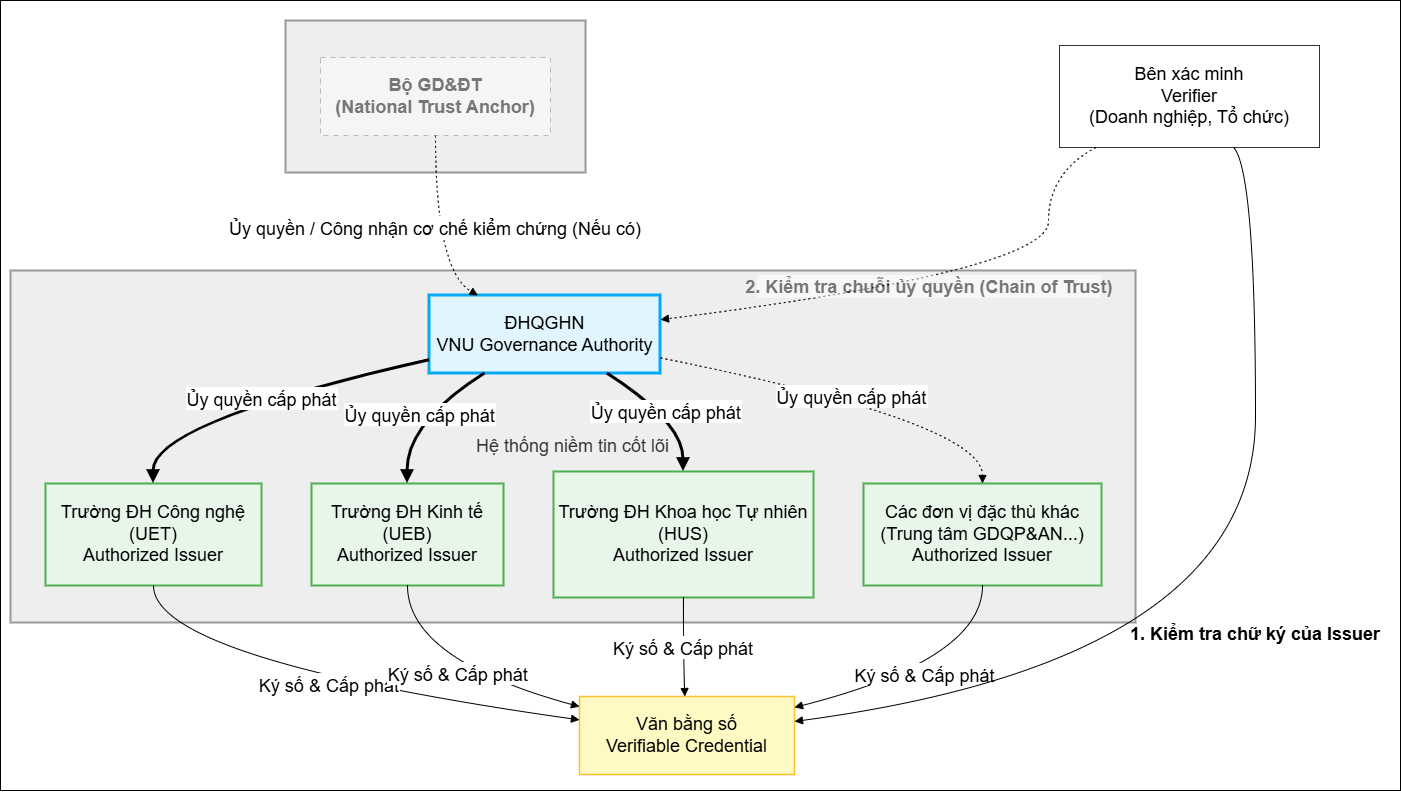
\includegraphics[width=0.88\textwidth]{images/trust-propagation-model.png}
    \caption{Mô hình lan truyền niềm tin theo cấu trúc phân cấp trong hệ thống văn bằng số}
    \label{fig:trust-propagation-model}
\end{figure}

\subsection{Sổ đăng ký tin cậy và yêu cầu đối với khung quản trị}

Thành phần hiện thực hóa tầng niềm tin thứ hai và thứ ba là \textbf{sổ đăng ký tin cậy} (trust registry) --- cơ chế lưu trữ và công bố trạng thái tin cậy của các bên phát hành trong hệ thống. Sổ đăng ký quản lý các thông tin: định danh của bên phát hành, trạng thái hiệu lực, phạm vi cấp phát được phép, thời hạn ủy quyền và quan hệ ủy quyền giữa các tổ chức. Theo nghĩa đó, nó là cầu nối giữa niềm tin kỹ thuật và niềm tin thể chế.

Khái niệm này đã được chuẩn hóa. Trust over IP Foundation công bố đặc tả Trust Registry Query Protocol phiên bản 2.0 vào tháng 4/2026 \cite{ToIP_TRQP2026}, định nghĩa một giao thức chỉ đọc để truy vấn dữ liệu có thẩm quyền từ các sổ đăng ký. Đặc tả xác định trường hợp sử dụng cốt lõi chính là câu hỏi đang xét: xác nhận rằng một bên phát hành được phép cấp một loại chứng thực cụ thể. Phiên bản 2.0 định nghĩa hai loại truy vấn --- truy vấn về thẩm quyền (authorization) và truy vấn về sự công nhận giữa các sổ đăng ký (recognition) --- và hoãn hai loại truy vấn khác, trong đó có truy vấn về ủy quyền nhiều cấp (delegation), sang phiên bản sau. Việc chính đặc tả chuẩn hóa còn hoãn phần ủy quyền nhiều cấp cho thấy đây là nội dung còn mở, và đó là một trong những điểm mà nghiên cứu này đóng góp.

Từ các phân tích trên, một khung quản trị niềm tin cần đáp ứng năm đặc tính:

\begin{itemize}
    \item \textbf{Tra cứu độc lập.} Trạng thái của bên phát hành phải tra cứu được mà không cần liên hệ bên phát hành hay cơ quan quản trị.
    \item \textbf{Lan truyền nhất quán.} Thay đổi về thẩm quyền phải có hiệu lực ngay trong các lần xác minh tiếp theo, không phụ thuộc vào việc bên xác minh có được thông báo hay không.
    \item \textbf{Phạm vi tường minh.} Thẩm quyền phải biểu diễn được theo phạm vi cụ thể, chứ không chỉ ở dạng nhị phân {``}được tin cậy / không được tin cậy{''}.
    \item \textbf{Dấu vết kiểm toán.} Mọi thay đổi quản trị phải để lại dấu vết không thể xóa, kể cả bởi chính cơ quan quản trị.
    \item \textbf{Phân tách khỏi lớp xác minh.} Thay đổi về quản trị không được đòi hỏi thay đổi ở phía bên xác minh.
\end{itemize}

Một đặc tính thứ sáu được các nghiên cứu gần đây nhấn mạnh và đáng được nêu, dù nằm ngoài phạm vi triển khai của khóa luận: trạng thái quản trị cần ở dạng \textbf{máy đọc được}, để ví và các tác nhân phần mềm tự động hóa được quyết định tin cậy thay vì đòi hỏi người dùng tự phán xét \cite{Weigl2025}. Yêu cầu này quan trọng vì nếu bên xác minh phải tự đọc và diễn giải một văn bản chính sách thì lớp quản trị không khác gì quy trình hành chính được số hóa. Trong thiết kế ở Chương 3, trạng thái thẩm quyền là dữ liệu có cấu trúc trên chuỗi nên thỏa mãn đặc tính này ở mức dữ liệu; phần chưa có là một biểu diễn máy đọc được cho \emph{chính sách} quản trị --- tức các quy tắc về điều kiện được cấp thẩm quyền, vốn hiện nằm ngoài hệ thống.

Năm đặc tính này trở thành tiêu chí thiết kế của khung quản trị được đề xuất ở Chương 3 và là căn cứ đối chiếu khi khảo sát các hệ thống hiện có.

\section{Khảo sát các hệ thống và giải pháp tiêu biểu}

Phần này phân tích các hệ thống tiêu biểu dưới lăng kính ba tầng niềm tin, nhằm xác định mỗi hệ thống giải quyết được tầng nào và để trống tầng nào.

\subsection{Blockcerts}

Blockcerts là một trong những hệ thống đầu tiên ứng dụng blockchain vào xác minh văn bằng, khởi nguồn từ MIT Media Lab \cite{Blockcerts2016}. Hệ thống biểu diễn chứng thực bằng JSON-LD, ký bằng khóa riêng của bên phát hành và neo giá trị băm của chứng thực lên một blockchain công khai.

Đóng góp lớn nhất của Blockcerts nằm ở tầng niềm tin kỹ thuật, và đóng góp đó mang tính lịch sử: hệ thống chứng minh được rằng xác minh độc lập hoàn toàn khả thi trong thực tế, ở quy mô thật, trước khi các chuẩn W3C đạt độ chín. Bên xác minh tự kiểm tra được chữ ký và tính toàn vẹn mà không cần liên hệ bên phát hành.

Tuy nhiên Blockcerts hầu như không giải quyết hai tầng còn lại. Hệ thống không có sổ đăng ký tin cậy hay cơ chế nào xác định tổ chức nào có thẩm quyền cấp phát; bất kỳ tổ chức nào cũng có thể sinh khóa và phát hành chứng thực {``}hợp lệ{''} về mặt kỹ thuật. Cơ chế thu hồi dựa vào danh sách do chính bên phát hành duy trì, nên bài toán quản trị ở quy mô hệ sinh thái vẫn còn nguyên. Đối chiếu với năm đặc tính ở Mục 2.6.3, Blockcerts đáp ứng đặc tính tra cứu độc lập đối với bản thân chứng thực nhưng không đáp ứng ba đặc tính liên quan tới thẩm quyền.

\noindent \textbf{Khoảng trống về thẩm quyền không phải một nhận xét lý thuyết}

Phần trên là một phân tích thiết kế, và một phân tích thiết kế có thể bị phản bác bằng lập luận rằng khoảng trống đó không gây hậu quả thực tế. Hai công trình phân tích an toàn cho thấy nó gây hậu quả thực tế, và cùng chỉ về một nguyên nhân gốc.

Baldi và cộng sự rà soát quy trình xác minh của Blockcerts và phát hiện một \textbf{tấn công mạo danh} \cite{Baldi2019}. Nguyên nhân nằm ở chỗ quy trình xác minh đối chiếu danh tính của bên phát hành với một \emph{hồ sơ bên phát hành không được xác thực}, lấy trực tuyến từ một địa chỉ do chính bên phát hành công bố. Kẻ tấn công vì vậy có thể dựng một hồ sơ bên phát hành giả cùng một chứng thực được sửa tương ứng, sao cho chứng thực giả \emph{không phân biệt được} với chứng thực thật bằng chính quy trình xác minh của hệ thống. Đáng chú ý là biện pháp khắc phục mà các tác giả đề xuất: tích hợp một hạ tầng khóa công khai cổ điển hoặc một hệ thống định danh phi tập trung --- nghĩa là bổ sung đúng lớp ràng buộc danh tính tổ chức mà hệ thống còn thiếu.

Bảy năm sau, cùng nhóm nghiên cứu báo cáo một \textbf{tấn công giả mạo} trên Block.co, một hệ thống chứng nhận văn bằng trên chuỗi đang được thương mại hóa, trong đó kẻ tấn công tạo được chứng thực giả mà hệ thống chấp nhận là hợp lệ \cite{Zonneveld2026}. Nguyên nhân gốc mà các tác giả xác định là việc \emph{thiếu một cơ quan có thẩm quyền được tin cậy}, khiến không thể ràng buộc danh tính pháp lý của một tổ chức với danh tính số của bên phát hành thuộc tổ chức đó; họ mô tả đây là một giới hạn nội tại của cách tiếp cận chứng nhận trên chuỗi và cảnh báo rằng các hệ thống tương tự có thể cũng dễ bị tấn công theo cách này.

Hai kết quả này có ý nghĩa trực tiếp đối với định hướng của khóa luận. Chúng cho thấy khoảng trống ở tầng niềm tin thể chế không phải một thiếu sót về sự hoàn chỉnh của mô hình mà là một \textbf{lớp lỗ hổng khai thác được}, và rằng việc bổ sung thêm cơ chế mật mã không lấp được nó --- cả hai hệ thống bị tấn công đều có chữ ký số hợp lệ và giá trị băm neo trên chuỗi đúng cách. Điều thiếu là một cơ chế để bên xác minh biết rằng \emph{khóa này thuộc về tổ chức có thẩm quyền đó}, và cơ chế đó thuộc phạm trù quản trị chứ không phải mật mã.

\subsection{Hạ tầng văn bằng số châu Âu: EDC và EBSI}

Liên minh Châu Âu phát triển hai thành phần bổ trợ nhau: European Digital Credentials for Learning cùng mô hình dữ liệu European Learning Model \cite{EDC_ELM} ở tầng chứng thực, và European Blockchain Services Infrastructure \cite{EBSI_TrustModel} ở tầng neo và quản trị.

Khác với Blockcerts, hệ thống này giải quyết đầy đủ cả ba tầng, và cách giải quyết tầng thứ ba đặc biệt đáng tham khảo. Mô hình niềm tin của EBSI xây dựng trên khái niệm \emph{tổ chức kiểm định được tin cậy}: các tổ chức này công nhận các bên phát hành cho một lĩnh vực và một phạm vi địa lý cụ thể, và bản thân sự công nhận đó cũng là một chứng thực có thể xác minh. Trong giáo dục, một bộ giáo dục quốc gia công nhận các trường đại học. Đồng thời, lược đồ của từng loại chứng thực được đăng ký trong một sổ đăng ký lược đồ riêng, nên bên xác minh kiểm tra được ba điều: định danh của bên phát hành, sự công nhận dành cho bên đó, và việc chứng thực có tuân theo lược đồ đã đăng ký.

Hai quan sát từ tài liệu kỹ thuật của EBSI có giá trị trực tiếp cho nghiên cứu này. Thứ nhất, sổ cái ghi nhận các quyết định về niềm tin nhưng không tạo ra chúng --- quyết định vẫn thuộc về cơ quan quản lý hoặc tổ chức kiểm định. Thứ hai, mỗi bên xác minh tự quyết định họ chấp nhận gốc niềm tin nào và theo chính sách nào. Hai nguyên tắc này được kế thừa trong thiết kế ở Chương 3.

Điểm mạnh khác của hệ thống châu Âu là sự gắn kết với hạ tầng pháp lý. Chứng thực không chỉ hợp lệ về mặt mật mã mà có giá trị pháp lý trong phạm vi Liên minh nhờ tích hợp với khung eIDAS \cite{eIDAS2014}, và khung này đã được sửa đổi năm 2024 để thiết lập Ví Định danh số Châu Âu \cite{eIDAS2_2024}, trong đó mỗi quốc gia thành viên có nghĩa vụ cung cấp ít nhất một ví vào cuối năm 2026.

Hạn chế của mô hình này là nó đánh đổi mức độ phi tập trung để lấy khả năng quản trị. Toàn bộ hệ sinh thái phụ thuộc mạnh vào hạ tầng và cơ chế quản trị của Liên minh, khiến nó khó áp dụng trực tiếp cho bối cảnh ngoài khối. Người học cũng có quyền kiểm soát hạn chế hơn, do dữ liệu chủ yếu nằm trên hạ tầng nền tảng thay vì trong ví cá nhân.

\subsection{Open Badges phiên bản 3.0}

Open Badges được thiết kế cho các chứng nhận vi mô và thành tích học tập linh hoạt. Phiên bản 3.0, được 1EdTech thông qua tháng 5/2024 \cite{OpenBadges2024}, đã tái cấu trúc để biểu diễn huy hiệu dưới dạng Verifiable Credential theo mô hình dữ liệu W3C, qua đó giải quyết tốt tầng niềm tin kỹ thuật.

Điểm mạnh của Open Badges là khả năng tổng hợp nhiều loại thành tích từ nhiều nguồn vào cùng một hồ sơ của người học, phù hợp với học tập mở và các chương trình đào tạo ngắn hạn. Tuy nhiên tầng niềm tin thể chế vẫn yếu: giá trị của một huy hiệu phụ thuộc chủ yếu vào uy tín xã hội của bên phát hành, và hệ thống không có sổ đăng ký tin cậy hay khung quản trị thống nhất để kiểm soát chất lượng bên phát hành. Đây là lựa chọn phù hợp với mục đích của chuẩn --- chứng nhận vi mô cần sự linh hoạt hơn là sự kiểm soát --- nhưng không đáp ứng yêu cầu của văn bằng đại học chính quy, nơi thẩm quyền cấp phát và sự công nhận pháp lý là điều kiện bắt buộc.

\subsection{Kiến trúc tham chiếu Trust over IP}

Trust over IP Foundation không phải một hệ thống triển khai mà là một kiến trúc tham chiếu cho hệ sinh thái định danh phi tập trung \cite{ToIP_Stack2022}. Đóng góp quan trọng nhất của kiến trúc này chính là nhận thức rằng niềm tin kỹ thuật không đủ để tạo niềm tin ở quy mô hệ sinh thái.

Phiên bản hiện hành của kiến trúc tổ chức tầng kỹ thuật thành bốn lớp: \emph{Trust Support} chứa các thành phần nền tảng như mô-đun tính toán tin cậy, lưu trữ an toàn và các sổ đăng ký dữ liệu có thể xác minh; \emph{Trust Spanning} thiết lập kết nối tin cậy giữa hai điểm cuối bằng một giao thức thống nhất, giữ vai trò tương tự lớp IP trong chồng giao thức TCP/IP; \emph{Trust Tasks} gồm các tác vụ nguyên tử như cấp phát và trình bày chứng thực; \emph{Trust Applications} là các ứng dụng gọi tới hai lớp dưới để thiết lập kết nối tin cậy.

Điểm đáng chú ý nhất về mặt phương pháp là cách kiến trúc xử lý vấn đề quản trị. Thay vì đặt quản trị thành một lớp riêng ở trên cùng, Trust over IP mô tả một \emph{chồng quản trị} song song với chồng kỹ thuật, trong đó siêu mô hình quản trị áp dụng được ở cả bốn lớp \cite{ToIP_GovMetamodel2022}. Cách nhìn này chính xác hơn: quản trị không phải một tầng chức năng mà là một chiều xuyên suốt của hệ thống. Thiết kế ở Chương 3 kế thừa quan điểm này ở mức nguyên tắc, dù vẫn trình bày quản trị thành một lớp riêng để giữ sự rõ ràng trong mô tả.

Hạn chế của Trust over IP là nó dừng ở mức kiến trúc tham chiếu. Nó không áp đặt blockchain, phương thức DID hay lược đồ cụ thể, và không cung cấp một mô hình triển khai cho lĩnh vực giáo dục; mỗi hệ sinh thái vẫn phải tự xây dựng khung quản trị phù hợp với bối cảnh của mình.

\subsection{EduCTX và các công trình học thuật liên quan}

EduCTX của Turkanović và cộng sự \cite{Turkanovic2018} là một trong những đề xuất học thuật có ảnh hưởng về nền tảng tín chỉ liên trường trên blockchain. Công trình xác định rõ bài toán liên thông định danh trong môi trường giáo dục đa cơ sở --- vấn đề thứ hai trong ba vấn đề của nghiên cứu này --- và đề xuất mô hình biểu diễn tín chỉ học tập dưới dạng token. Hạn chế là mô hình tập trung vào việc biểu diễn và chuyển đổi tín chỉ hơn là vào bài toán thẩm quyền cấp phát.

Các khảo sát hệ thống gần đây cho thấy khoảng trống về quản trị là đặc điểm chung của cả lĩnh vực. Rà soát 63 bài báo giai đoạn 2018--2023 về quản trị trong kiểm định giáo dục trên nền blockchain, De Alwis và cộng sự kết luận rằng tài liệu hiện có hầu như không có đề xuất nào về một khung quản trị, trong khi ở mô hình truyền thống chính khung quản trị mới là yếu tố bảo đảm tính xác thực của văn bằng \cite{DeAlwis2025}. Báo cáo chính sách của Trung tâm Nghiên cứu Chung thuộc Ủy ban Châu Âu về blockchain trong giáo dục cũng nêu bật rằng các rào cản chính không nằm ở công nghệ mà ở quản trị và tiêu chuẩn hóa \cite{Grech2017}. Ở phía định danh, các khảo sát của Mühle và cộng sự \cite{Muhle2018} cùng Schardong và Custódio \cite{Schardong2022} xác nhận rằng cơ chế thiết lập niềm tin ở mức hệ sinh thái là một trong những thành phần ít được giải quyết nhất của các hệ thống định danh tự chủ.

\subsection{Bối cảnh Việt Nam}

Tại Việt Nam, hạ tầng liên quan đang hình thành nhanh. Nền tảng blockchain quốc gia NDAChain, ra mắt năm 2025, được thiết kế như một lớp hạ tầng trung gian để xác thực và ghi nhận giao dịch dữ liệu, theo mô hình được cấp phép với tập nút xác thực được lựa chọn và giám sát; nền tảng đi kèm một giải pháp định danh phi tập trung và một ứng dụng quản lý định danh \cite{NDAChain2025}. Khung kiến trúc tổng thể quốc gia số công bố tháng 10/2025 xác định blockchain quốc gia là hạ tầng số dùng chung. Song song, hệ thống định danh điện tử công dân đã đạt độ phủ rộng và theo Thông tư 10/2026/TT-BGDĐT \cite{TT10_2026}, việc tra cứu văn bằng trên nền tảng này có thể thay thế bản sao từ sổ gốc.

Đặc điểm của bối cảnh này là các khối hạ tầng đã có nhưng lớp quản trị thẩm quyền cấp phát trong lĩnh vực giáo dục thì chưa được định hình. Đây là lý do nghiên cứu thiết kế khung quản trị độc lập với nền tảng neo cụ thể: mô hình thẩm quyền có thể chuyển sang một hạ tầng khác mà không cần thiết kế lại, miễn hạ tầng đó cung cấp ba tính chất đã nêu ở Mục 2.5.1.

\subsection{Tổng hợp khảo sát}

\begin{longtable}{|p{2.4cm}|p{2.5cm}|p{3.1cm}|p{3.1cm}|p{2.6cm}|}
\caption{Tổng hợp khảo sát các hệ thống tiêu biểu theo ba tầng niềm tin}
\label{tab:trust-layer-survey} \\

\hline
\textbf{Hệ thống} &
\textbf{Niềm tin kỹ thuật} &
\textbf{Niềm tin thể chế} &
\textbf{Niềm tin quản trị} &
\textbf{Holder giữ dữ liệu} \\
\hline
\endfirsthead

\hline
\textbf{Hệ thống} &
\textbf{Niềm tin kỹ thuật} &
\textbf{Niềm tin thể chế} &
\textbf{Niềm tin quản trị} &
\textbf{Holder giữ dữ liệu} \\
\hline
\endhead

\hline
\endfoot

\hline
\endlastfoot

Blockcerts
& Đầy đủ: chữ ký và băm neo trên chuỗi
& Không có. Khoảng trống này đã bị khai thác: tấn công mạo danh qua hồ sơ bên phát hành không được xác thực \cite{Baldi2019}
& Không có: thu hồi dựa trên danh sách do bên phát hành tự giữ
& Có
\\ \hline

EDC / EBSI
& Đầy đủ
& Đầy đủ: tổ chức kiểm định công nhận bên phát hành theo lĩnh vực và địa bàn
& Đầy đủ nhưng tập trung: phụ thuộc hạ tầng và quản trị của Liên minh
& Hạn chế: dữ liệu chủ yếu trên hạ tầng nền tảng
\\ \hline

Open Badges 3.0
& Đầy đủ sau khi tích hợp mô hình dữ liệu W3C
& Yếu: giá trị phụ thuộc uy tín xã hội của bên phát hành
& Không có sổ đăng ký hay khung quản trị thống nhất
& Có
\\ \hline

Trust over IP
& Mô tả ở mức kiến trúc tham chiếu
& Mô tả: chồng quản trị song song chồng kỹ thuật
& Mô tả đầy đủ nhất về khái niệm, không có triển khai cho giáo dục
& Theo thiết kế
\\ \hline

EduCTX
& Đầy đủ cho biểu diễn tín chỉ
& Không phải trọng tâm của công trình
& Không đề cập cơ chế thu hồi thẩm quyền
& Có
\\ \hline

Mô hình đề xuất
& Đầy đủ, kèm bước đối chiếu nội dung với băm đã neo
& Chuỗi thẩm quyền đặc tả thành mã thi hành, có phạm vi và thời hạn
& Trạng thái quản trị công khai trên chuỗi, dấu vết không thể xóa
& Có: ví không lưu ký
\\ \hline

\end{longtable}


\section{Khoảng trống nghiên cứu}

\subsection{Phân loại khoảng trống theo tầng}

Khảo sát ở Mục 2.7 cho phép xác định khoảng trống cụ thể hơn so với phát biểu chung {``}thiếu quản trị niềm tin{''}. Tuy nhiên, nếu chỉ liệt kê các khoảng trống ở dạng danh sách ngang hàng thì không đánh giá được chúng thuộc loại nào và một nghiên cứu đơn lẻ có thể xử lý tới đâu --- một khoảng trống ở tầng chuẩn hóa đòi hỏi quá trình đồng thuận của cả cộng đồng, trong khi một khoảng trống ở tầng kiến trúc có thể xử lý trong phạm vi một hệ thống.

Vì vậy phần này phân loại khoảng trống thành sáu tầng, mỗi tầng kèm bằng chứng từ tài liệu và phạm vi xử lý của nghiên cứu này. Bảng \ref{tab:gap-taxonomy} tổng hợp, và các mục dưới đây phân tích từng tầng.

\begin{longtable}{|c|p{2.9cm}|p{4.4cm}|p{2.5cm}|p{2.6cm}|}
\caption{Phân loại khoảng trống nghiên cứu theo tầng và phạm vi can thiệp của khóa luận}
\label{tab:gap-taxonomy} \\

\hline
\textbf{Mã} & \textbf{Tầng} & \textbf{Nội dung khoảng trống} & \textbf{Bằng chứng} & \textbf{Khóa luận xử lý} \\
\hline
\endfirsthead

\hline
\textbf{Mã} & \textbf{Tầng} & \textbf{Nội dung khoảng trống} & \textbf{Bằng chứng} & \textbf{Khóa luận xử lý} \\
\hline
\endhead

\hline
\endfoot

\hline
\endlastfoot

G1 & Chuẩn hóa
& Chuẩn về truy vấn sổ đăng ký tin cậy còn hoãn phần ủy quyền nhiều cấp; chuẩn về trạng thái chứng thực không biểu diễn thẩm quyền
& \cite{ToIP_TRQP2026}, \cite{W3C_BitstringStatusList2025}
& \textbf{Góp một điểm dữ liệu}: đưa ra cách biểu diễn cụ thể và chứng minh nó chạy được
\\ \hline

G2 & Kiến trúc
& Lớp quản trị khi tồn tại thường là cơ sở dữ liệu do một tổ chức vận hành, nên chỉ \emph{di chuyển} sự phụ thuộc vào trung gian chứ không loại bỏ
& \cite{Baldi2019}, \cite{Zonneveld2026}, \cite{SSI_Survey2025}
& \textbf{Xử lý trực tiếp}: sổ đăng ký là trạng thái hợp đồng trên chuỗi công khai
\\ \hline

G3 & Biểu diễn thẩm quyền
& Thẩm quyền biểu diễn ở dạng nhị phân; thiếu ba chiều phạm vi, thời hạn và số cấp ủy quyền
& \cite{Blockcerts2016}, \cite{OpenBadges2024}, \cite{ToIP_TRQP2026}
& \textbf{Xử lý trực tiếp}: mặt nạ bit, trường thời hạn, ủy quyền hai cấp có ràng buộc
\\ \hline

G4 & Ngữ nghĩa xác minh
& Quy trình xác minh không phân biệt loại thất bại; nhiều hệ thống không đối chiếu nội dung với giá trị băm đã neo
& Mục 2.7.1, Mục 2.7.3
& \textbf{Xử lý trực tiếp}: bảy bước có báo cáo riêng, gồm bước đối chiếu nội dung
\\ \hline

G5 & Phương pháp đánh giá
& Lĩnh vực thiếu nghiên cứu người dùng: chỉ 2 trong 47 công trình được phân tích có đánh giá tính khả dụng; các khung niềm tin chỉ kiểm chứng bằng cài đặt hợp đồng
& \cite{Ambati2026}, \cite{DeSalve2023}
& \textbf{Không xử lý} --- khóa luận nằm trong cùng giới hạn này; thừa nhận tại Mục 4.11 và Mục 5.3
\\ \hline

G6 & Bối cảnh
& Tại Việt Nam, hành lang pháp lý và hạ tầng số đã hình thành nhưng chưa có lớp quản trị thẩm quyền cấp phát cho lĩnh vực giáo dục
& \cite{TT10_2026}, \cite{LuatBVDLCN2025}, \cite{NDAChain2025}
& \textbf{Xử lý một phần}: trong phạm vi một trường hợp nghiên cứu
\\ \hline

\end{longtable}


\noindent \textbf{G1 --- Khoảng trống ở tầng chuẩn hóa}

Các đặc tả hiện hành chưa bao phủ đầy đủ việc biểu diễn thẩm quyền. Đặc tả Trust Registry Query Protocol phiên bản 2.0 định nghĩa hai loại truy vấn --- về thẩm quyền và về sự công nhận lẫn nhau giữa các sổ đăng ký --- nhưng \textbf{hoãn loại truy vấn về ủy quyền nhiều cấp sang phiên bản sau} \cite{ToIP_TRQP2026}. Ở phía trạng thái chứng thực, cơ chế danh sách bit của W3C \cite{W3C_BitstringStatusList2025} giải quyết rất tốt bài toán trạng thái nhưng không biểu diễn thẩm quyền của bên phát hành; hai bài toán này được chuẩn hóa độc lập và chưa có cơ chế gắn kết chúng.

Đây là khoảng trống mà một khóa luận \emph{không thể lấp}, vì việc chuẩn hóa thuộc về quá trình đồng thuận của cộng đồng. Điều nghiên cứu này có thể làm là đưa ra một cách biểu diễn cụ thể cho phần còn hoãn và chứng minh nó chạy được, qua đó đóng góp một điểm dữ liệu cho quá trình chuẩn hóa.

\noindent \textbf{G2 --- Khoảng trống ở tầng kiến trúc}

Khi lớp quản trị tồn tại, nó thường được hiện thực hóa bằng một cơ sở dữ liệu do một tổ chức vận hành. Hạ tầng văn bằng số châu Âu là ví dụ hoàn chỉnh nhất của hướng này \cite{EBSI_TrustModel}, và nó hoạt động tốt trong phạm vi có một cơ quan quản trị được công nhận.

Quan sát quan trọng là: cách làm đó \textbf{di chuyển} sự phụ thuộc vào trung gian chứ không loại bỏ nó. Bên xác minh không còn phải tin cơ sở cấp phát, nhưng phải tin tổ chức vận hành sổ đăng ký. Khảo sát tổng quan về định danh tự chủ ghi nhận rủi ro tập trung hóa bên phát hành như một nguy cơ quản trị có thể tạo ra điểm hỏng đơn lẻ \cite{SSI_Survey2025}. Đây là khoảng trống mà nghiên cứu này xử lý trực tiếp: đặt sổ đăng ký thành trạng thái của một hợp đồng trên chuỗi công khai.

Cần ghi nhận rằng hướng này đã có công trình đi trước. Eer, Diaz và Kohlweiss đề xuất một sổ đăng ký tin cậy theo hướng từ dưới lên, dựa trên uy tín và kèm cơ chế khuyến khích tham gia trung thực \cite{Eer2022}; De Salve và cộng sự đề xuất một khung niềm tin nhiều lớp dựa trên quan hệ tin cậy giữa các tác nhân, cài đặt bằng hợp đồng thông minh \cite{DeSalve2023}. Hai công trình này giải quyết câu hỏi {``}bên xác minh nên tin ai{''} theo hướng \emph{uy tín phân tán}; nghiên cứu này giải quyết theo hướng \emph{ủy quyền thể chế có cấu trúc}. Hai hướng bổ trợ nhau và phù hợp với hai loại hệ sinh thái khác nhau: hướng uy tín phù hợp khi không có cơ quan quản trị được công nhận, hướng ủy quyền phù hợp khi có --- và trong giáo dục đại học thì luôn có.

\noindent \textbf{G3 --- Khoảng trống ở tầng biểu diễn thẩm quyền}

Phần lớn hệ thống biểu diễn thẩm quyền ở dạng nhị phân: một bên phát hành được tin cậy hoặc không. Ba chiều thông tin bị thiếu, và cả ba đều có trong thực tiễn quản trị giáo dục:

\begin{itemize}
    \item \textbf{Phạm vi.} Một trường được kiểm định cho một số ngành và trình độ nhất định, không phải cho mọi loại văn bằng.
    \item \textbf{Thời hạn.} Thẩm quyền gắn với một chu kỳ kiểm định và tự hết hiệu lực nếu không được gia hạn.
    \item \textbf{Số cấp.} Một trường được ủy quyền có thể cần ủy quyền tiếp cho một đơn vị trực thuộc.
\end{itemize}

Hạ tầng châu Âu xử lý được hai chiều đầu thông qua khái niệm tổ chức kiểm định công nhận bên phát hành theo lĩnh vực và địa bàn \cite{EBSI_TrustModel}. Chiều thứ ba thì, như đã nêu ở G1, còn hoãn ngay ở tầng chuẩn hóa. Đây là khoảng trống mà nghiên cứu này xử lý đầy đủ nhất.

\noindent \textbf{G4 --- Khoảng trống ở tầng ngữ nghĩa của quy trình xác minh}

Khi một chứng thực bị từ chối, bên xác minh cần biết nguyên nhân là nội dung bị sửa, hay chứng thực đã bị thu hồi, hay bên phát hành đã mất thẩm quyền --- ba tình huống đòi hỏi ba cách xử lý hoàn toàn khác nhau. Một kết quả {``}không hợp lệ{''} chung không đủ để hành động.

Liên quan tới đây là một khoảng trống cụ thể hơn: nhiều hệ thống kiểm trạng thái chứng thực nhưng không đối chiếu \emph{nội dung} với giá trị băm đã neo, nên không phát hiện được trường hợp nội dung bị sửa sau khi cấp. Mục 3.6.1 và Mục 4.8.3 phân tích và kiểm chứng điểm này.

\noindent \textbf{G5 --- Khoảng trống ở tầng phương pháp đánh giá}

Đây là khoảng trống mà nghiên cứu này \emph{cũng mắc phải}, nên cần nêu trung thực. Khảo sát hệ thống của Ambati và cộng sự trên 80 nguồn, trong đó phân tích 47 công trình khoa học và 12 hệ thống đang vận hành, ghi nhận rằng chỉ \textbf{2 trong 47} công trình có nghiên cứu người dùng hoặc đánh giá tính khả dụng, và gọi đây là một khoảng trống nghiêm trọng của lĩnh vực \cite{Ambati2026}. Các khung niềm tin được đề xuất thường được kiểm chứng bằng cách cài đặt hợp đồng thông minh và đo hiệu năng \cite{DeSalve2023}, chứ không bằng nghiên cứu người dùng hay triển khai thực địa.

Trong số rất ít nghiên cứu người dùng đã có, nghiên cứu của Zaeem và cộng sự ghi nhận rằng quá trình khởi tạo gây khó hiểu và người dùng lo lắng về việc mất khóa riêng \cite{Zaeem2021} --- đúng hai vấn đề mà mô hình ví không lưu ký ở Mục 2.3.4 đặt ra. Nghiên cứu này ở trong đúng nhóm thiếu bằng chứng đó: nó kiểm chứng bằng bộ kiểm thử và phép đo hiệu năng, không có nghiên cứu người dùng. Việc đặt khoảng trống này thành một tầng riêng có hai mục đích: thừa nhận giới hạn của kết quả thu được (Mục 4.11), và xác định rõ rằng kết luận của khóa luận là về \emph{tính khả thi kỹ thuật}, không phải về \emph{mức độ tiếp nhận}. Nghiên cứu phỏng vấn về yếu tố quyết định mức độ tiếp nhận định danh tự chủ cho thấy hai câu hỏi này tách biệt và không suy ra được từ nhau \cite{SSI_Adoption2025}.

\noindent \textbf{G6 --- Khoảng trống ở tầng bối cảnh}

Khoảng trống này mang tính địa phương nhưng là lý do trực tiếp của đề tài. Tại Việt Nam, ba điều kiện đã hội đủ: hành lang pháp lý công nhận giá trị pháp lý của văn bằng số \cite{TT10_2026}, quy định về bảo vệ dữ liệu cá nhân đặt ra ràng buộc kiến trúc rõ ràng \cite{LuatBVDLCN2025}, và hạ tầng số quốc gia gồm nền tảng blockchain và giải pháp định danh phi tập trung đang được triển khai \cite{NDAChain2025}.

Điều còn thiếu là lớp quản trị thẩm quyền cấp phát trong lĩnh vực giáo dục: chưa có cơ chế nào cho phép một bên thứ ba kiểm chứng rằng một đơn vị được phép cấp một loại văn bằng cụ thể. Các hạ tầng nêu trên cung cấp nền neo và nền định danh, nhưng không tự sinh ra lớp quản trị đó --- nó phải được thiết kế riêng cho từng lĩnh vực, giống như hạ tầng châu Âu phải thiết kế riêng mô hình tổ chức kiểm định cho giáo dục.

\subsection{Định hướng của nghiên cứu}

Từ phân loại trên, phạm vi can thiệp của khóa luận được xác định như sau. Nghiên cứu xử lý \textbf{trực tiếp} ba tầng G2, G3 và G4, là ba tầng thuộc phạm vi kiến trúc và có thể kiểm chứng trong một hệ thống đơn lẻ. Nghiên cứu \textbf{đóng góp một điểm dữ liệu} cho G1 bằng cách đưa ra một cách biểu diễn cụ thể cho phần mà chuẩn còn hoãn và chứng minh nó chạy được. Nghiên cứu \textbf{xử lý một phần} G6 trong phạm vi một trường hợp nghiên cứu. Và nghiên cứu \textbf{không xử lý} G5 --- nó nằm trong cùng giới hạn phương pháp mà G5 mô tả, và điều này được thừa nhận thay vì bỏ qua.

Hướng tiếp cận tương ứng: dùng các chuẩn mở về định danh phi tập trung và chứng thực có thể xác minh làm nền kỹ thuật, bảo đảm xác minh độc lập và quyền kiểm soát dữ liệu của người học; đồng thời xây dựng một khung quản trị niềm tin trong đó chuỗi thẩm quyền được đặc tả thành mã thi hành trên một hạ tầng công khai bất biến, với phạm vi và thời hạn tường minh, và quy trình xác minh phân biệt rõ các loại thất bại. Kiến trúc hiện thực hóa hướng tiếp cận này được trình bày ở Chương 3.
